% Second-order conjugate heat transfer at an immersed interface.
% Companion derivation for docs/next_session_conjugate.md.
% Build:  latexmk -pdf conjugate_ibm.tex   (or: make)
\documentclass[11pt,a4paper]{article}

\usepackage[T1]{fontenc}
\usepackage[utf8]{inputenc}
\usepackage{lmodern}
\usepackage[margin=2.6cm]{geometry}
\usepackage{amsmath,amssymb}
\usepackage{booktabs}
\usepackage{microtype}
\usepackage{tikz}
\usepackage{caption}
\usepackage[colorlinks=true,linkcolor=blue!50!black,citecolor=blue!50!black,
            urlcolor=blue!50!black]{hyperref}
\usetikzlibrary{arrows.meta,calc,patterns,decorations.pathmorphing,positioning}

\definecolor{solidcol}{RGB}{170,170,170}
\definecolor{fluidcol}{RGB}{235,245,255}
\definecolor{hot}{RGB}{200,60,40}
\definecolor{cold}{RGB}{40,90,190}

\newcommand{\jump}[1]{\left[#1\right]}
\newcommand{\dd}{\mathrm{d}}
\newcommand{\ed}{\boldsymbol{e}_d}
\newcommand{\nn}{\boldsymbol{n}}
\newcommand{\grad}{\boldsymbol{\nabla}}
\newcommand{\Rser}{\mathcal{R}}
\newcommand{\code}[1]{\texttt{#1}}

\title{Second-order conjugate heat transfer at an immersed\\
       fluid/solid interface in \textsc{mobydiff}\\[2mm]
       \large Combining the Luchini immersed-boundary correction with the\\
       explicit-jump immersed interface method}
\author{Design note --- companion to \code{docs/next\_session\_conjugate.md}}
\date{2026-08-03}

\begin{document}
\maketitle

\begin{abstract}
\noindent
We derive a discretisation for conjugate heat transfer (CHT) across an immersed,
generally non-grid-aligned fluid/solid interface that is second-order accurate in
the diffusive term, conservative by construction, fully explicit, and reduces
\emph{exactly} to the immersed-boundary correction of Luchini
et~al.~\cite{luchini2025} in the isothermal-body limit and to a zero-flux mask in
the adiabatic limit. The construction combines two ingredients: from
\cite{luchini2025} the idea that the presence of the boundary can be absorbed
into a \emph{local} modification of the diffusive operator alone, with the
across-interface unknown eliminated analytically; from the explicit-jump immersed
interface method (EJIIM) of Wiegmann \& Bube~\cite{ejiim2000} the jump-corrected
finite differences that make an oblique interface second-order accurate. The
central result is
\begin{equation*}
  F_{\text{face}}
   = \frac{T_R-T_L}{\Rser} \;+\; s_t\left(k_{\text{loc}}-\frac{h_d}{\Rser}\right),
  \qquad
  \Rser = \frac{\delta_L}{k_L}+\frac{\delta_R}{k_R},
\end{equation*}
a two-point series-resistance flux plus one tangential correction term. The
first term is the exact resummation of the normal-derivative jump; the second is
the EJIIM contribution and involves only the \emph{continuous} tangential
gradient, which is what makes the scheme robust at high conductivity contrast.
We also show why \cite{luchini2025} legitimately needs no tangential term for
Dirichlet boundaries, and why CHT does. Section~\ref{sec:coco} rederives the
same result from the corner-correction (COCO) viewpoint of Cipelli
et~al.~\cite{cipelli2025} --- matching the normal derivatives of two
complementary $180^\circ$ wedge solutions --- which supplies both an
independent check and the route to the one case the flat model cannot cover:
a \emph{conducting sharp corner}.

\medskip\noindent
\textbf{What to implement.} At DNS resolution the near-wall field is locally
one-dimensional, and the tangential term is small in a way that can be
\emph{measured} rather than assumed. Section~\ref{sec:baseline} is therefore the
recommended starting point and the practical heart of this note: keeping only
the series resistance, and evaluating it through the level-set fraction
$w=\varphi_L/(\varphi_L-\varphi_R)$ of the two cell-centre signed distances,
reduces conjugate heat transfer to \emph{one face coefficient} --- with no new
stored data, because the signed distance is the existing \code{dwall} field. The
interface obliquity cancels out of $w$ exactly (Sec.~\ref{sec:lemma}), the
error incurred is given in closed form and is computable at run time
(Sec.~\ref{sec:cost}), and the escalation back to the full
Eq.~\eqref{eq:main} is one extra term at the same face
(Sec.~\ref{sec:escalation}).
\end{abstract}

\tableofcontents

%======================================================================
\section{Problem statement}
%======================================================================

\subsection{Continuous equations}

Conjugate heat transfer means one temperature field $T$ defined over both the
fluid domain $\Omega_f$ and the solid domain $\Omega_s$, coupled at the immersed
interface $\Gamma=\partial\Omega_f\cap\partial\Omega_s$:
\begin{align}
  (\rho c)_f\left(\frac{\partial T}{\partial t}+\grad\!\cdot(\boldsymbol{u}T)\right)
    &= \grad\!\cdot\!\left(k_f\grad T\right) && \text{in }\Omega_f, \label{eq:fluid}\\
  (\rho c)_s\,\frac{\partial T}{\partial t}
    &= \grad\!\cdot\!\left(k_s\grad T\right) && \text{in }\Omega_s. \label{eq:solid}
\end{align}
The interface conditions are continuity of temperature and of normal heat flux,
\begin{equation}
  \jump{T}_\Gamma = 0,
  \qquad
  \jump{k\,\partial_n T}_\Gamma = 0,
  \label{eq:interface}
\end{equation}
where $\jump{\cdot}$ denotes the solid-side minus the fluid-side limit and
$\nn$ is the unit normal pointing from fluid into solid. A finite contact
resistance is the trivial generalisation $\jump{T}=R_c\,k_f\partial_nT$ and is
carried through the derivation at no cost (Sec.~\ref{sec:contact}).

Note carefully: \emph{both} material properties jump, and they jump in different
combinations. The interface condition~\eqref{eq:interface} involves the
\emph{conductivity} $k$; the transient behaviour involves the \emph{diffusivity}
$\alpha=k/(\rho c)$. A formulation that carries only $\alpha$ (as a naive reuse
of the existing scalar diffusivity would) cannot represent~\eqref{eq:interface}.

\subsection{Non-dimensional form matching the solver}

\textsc{mobydiff} advances cell-centred scalars with diffusivity
$1/(\mathrm{Re}\,\mathrm{Pr})$ (\code{scalar\_transport\_kernel}). Introduce the
two pointwise material ratios
\begin{equation}
  \kappa(\boldsymbol{x}) = \frac{k(\boldsymbol{x})}{k_f},
  \qquad
  C(\boldsymbol{x}) = \frac{(\rho c)(\boldsymbol{x})}{(\rho c)_f},
  \qquad
  \kappa \equiv C \equiv 1 \;\text{ in the fluid},
\end{equation}
so that \eqref{eq:fluid}--\eqref{eq:solid} become the single equation
\begin{equation}
  \frac{\partial T}{\partial t}
  = \frac{1}{C}\left[
      \frac{1}{\mathrm{Re}\,\mathrm{Pr}}\,\grad\!\cdot\!\left(\kappa\grad T\right)
      - \chi_f\,\grad\!\cdot(\boldsymbol{u}T)
    \right],
  \label{eq:onefield}
\end{equation}
with $\chi_f$ the fluid indicator. In the fluid $C=\kappa=1$ and
\eqref{eq:onefield} is \emph{exactly} the equation the existing kernel solves ---
which is the structural reason the feature can be bit-exact when disabled and
even when enabled away from the body. The solid is characterised by two
dimensionless numbers per scalar,
\begin{equation}
  \kappa_s = \frac{k_s}{k_f},
  \qquad
  C_s = \frac{(\rho c)_s}{(\rho c)_f},
  \qquad\text{whence}\qquad
  \frac{\alpha_s}{\alpha_f}=\frac{\kappa_s}{C_s}.
\end{equation}

\subsection{How to read this note}

The material is ordered by argument, not by implementation priority:
Secs.~\ref{sec:derivation}--\ref{sec:coco} derive the exact cut-face flux and
establish what formal second order requires;
Sec.~\ref{sec:baseline} then decides what to actually build at DNS resolution,
and Sec.~\ref{sec:cheaper} asks whether the problem can be avoided altogether.
An implementer in a hurry can read Sec.~\ref{sec:cheaper}, then
Sec.~\ref{sec:baseline}, then the discrete scheme, and treat the rest as the
justification for the two terms that appear there.

\subsection{Geometric setting}

Figure~\ref{fig:geometry} fixes the notation used throughout. The interface cuts
the segment joining two neighbouring cell centres; the cell whose \emph{centre}
lies in the fluid is fluid, the other solid. Such a segment is called a
\emph{cut arm}, and the corresponding cell face a \emph{cut face}.

\begin{figure}[htbp]
\centering
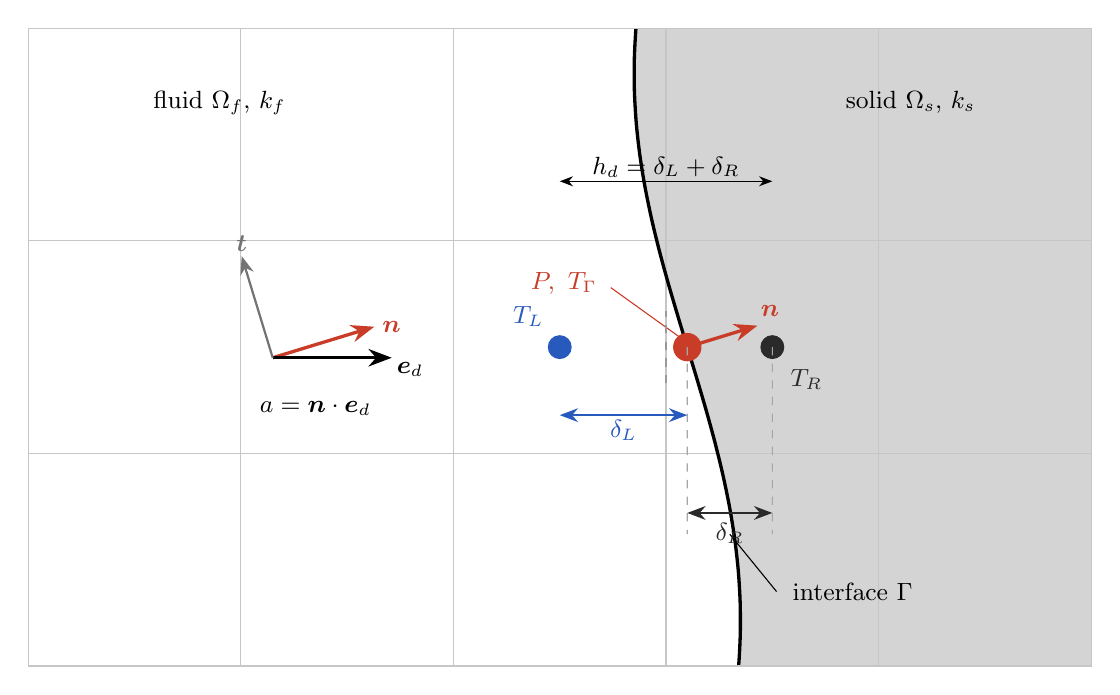
\begin{tikzpicture}[scale=2.7,>=Stealth,font=\small]
  \begin{scope}
    \clip (0,0) rectangle (5,3);
    \fill[solidcol,opacity=0.5]
       plot[domain=-0.3:3.3,smooth,variable=\y] ({3.1-0.25*sin(70*(\y-1.5))},\y)
       -- (5.3,3.3) -- (5.3,-0.3) -- cycle;
    \draw[gray!45] (0,0) grid[step=1] (5,3);
    \draw[very thick,black]
       plot[domain=-0.3:3.3,smooth,variable=\y] ({3.1-0.25*sin(70*(\y-1.5))},\y);
  \end{scope}
  \draw[gray!45] (0,0) rectangle (5,3);
  \node at (0.90,2.65) {fluid $\Omega_f$, $k_f$};
  \node at (4.15,2.65) {solid $\Omega_s$, $k_s$};
  \node[anchor=west] at (3.55,0.35) {interface $\Gamma$};
  \draw[thin,black] (3.52,0.35) -- (3.30,0.62);

  % direction triad, drawn as a legend in free space
  \begin{scope}[shift={(1.15,1.45)}]
    \draw[->,very thick,hot]   (0,0) -- (0.478,0.146) node[right=-1pt] {$\nn$};
    \draw[->,very thick,black] (0,0) -- (0.560,0)     node[below right=-3pt] {$\ed$};
    \draw[->,thick,black!55]   (0,0) -- (-0.146,0.478) node[above=-2pt] {$\boldsymbol{t}$};
    \node[anchor=north] at (0.20,-0.16) {$a=\nn\cdot\ed$};
  \end{scope}

  % cell centres on the row y = 1.5
  \coordinate (L) at (2.5,1.5);
  \coordinate (R) at (3.5,1.5);
  \coordinate (P) at (3.1,1.5);
  \fill[cold] (L) circle (1.6pt);
  \node[cold,anchor=south east] at (2.47,1.55) {$T_L$};
  \fill[solidcol!25!black] (R) circle (1.6pt);
  \node[solidcol!25!black,anchor=north west] at (3.54,1.44) {$T_R$};
  \fill[hot] (P) circle (1.9pt);
  \node[hot,anchor=east] at (2.72,1.80) {$P,\ T_\Gamma$};
  \draw[hot,thin] (2.74,1.78) -- (3.06,1.55);
  \draw[->,very thick,hot] (P) -- ++(0.33,0.101);
  \node[hot,anchor=south west] at (3.40,1.60) {$\nn$};

  % distances, staggered so no two labels share a line
  \draw[dashed,gray!70] (P) -- (3.1,0.62);
  \draw[dashed,gray!70] (R) -- (3.5,0.62);
  \draw[<->,thick,cold] (2.5,1.18) -- node[below=-2pt]{$\delta_L$} (3.1,1.18);
  \draw[<->,thick,solidcol!25!black] (3.1,0.72) -- node[below=0pt]{$\delta_R$} (3.5,0.72);
  \draw[<->] (2.5,2.28) -- node[above=-2pt]{$h_d=\delta_L+\delta_R$} (3.5,2.28);

  % cell face (midpoint of the L-R segment); here it falls on the fluid side
  \draw[dashed,gray!80] (3.0,1.33) -- (3.0,1.67);
\end{tikzpicture}
\caption{Cut arm and cut face. Cell centres $L$ (fluid) and $R$ (solid) straddle
the interface $\Gamma$, which crosses the connecting segment at $P$ at distances
$\delta_L$ and $\delta_R$ with $\delta_L+\delta_R=h_d$. The interface normal
$\nn$ at $P$ is in general \emph{not} aligned with the coordinate direction
$\ed$; the misalignment is measured by $a=\nn\cdot\ed$ (triad drawn as a legend
on the left). The short dashed tick marks the cell face, at the midpoint of the
$L$--$R$ segment; here it falls on the fluid side, so $k_{\text{loc}}=k_f$ in
Eq.~\eqref{eq:main}. All quantities are per arm: a cell may have up to six cut
arms.}
\label{fig:geometry}
\end{figure}

%======================================================================
\section{The two source methods}
%======================================================================

\subsection{Luchini et al.: the implicit Dirichlet immersed boundary}
\label{sec:luchini}

Consider a one-dimensional arm along $x$ in which the neighbour $x_{i-1}$ of a
fluid point $x_i$ lies inside the body, with the wall at distance $\delta$ from
$x_i$ and $\Delta$ the mesh spacing (Fig.~\ref{fig:luchini}). The staircase
approximation sets $w_{i-1}=0$ and is first-order. Reference~\cite{luchini2025}
instead \emph{linearly extrapolates} the ghost value through the first fluid
point and the true wall value (their Eqs.~4--5),
\begin{equation}
  w_{i-1} \;\longleftarrow\; \frac{\delta-\Delta}{\delta}\,w_i ,
  \label{eq:luchini-ghost}
\end{equation}
and---this is the crucial step---substitutes \eqref{eq:luchini-ghost} back into
the Laplacian instead of storing it. The whole effect of the boundary collapses
onto the \emph{centre weight} of the stencil (their Eqs.~6--7),
\begin{equation}
  \tilde d^{(2)}_{x;i}(0) = d^{(2)}_{x;i}(0) - \underbrace{d^{(2)}_{x;i}(-1)\,
    \frac{\Delta-\delta}{\delta}}_{\textstyle \equiv\,\lambda},
  \qquad
  \lambda \;=\; \nu\,\frac{\Delta-\delta}{\delta\,\Delta^{2}}
  \quad\text{(uniform mesh)} .
  \label{eq:lambda}
\end{equation}
This is precisely what \code{ibm.f90} stores: \code{add\_neighbor\_coeff}
accumulates $\big((d_0-d)/d\big)/d_0^{2}$ per arm and scales by $1/\mathrm{Re}$,
i.e.\ $(\Delta-\delta)/(\delta\Delta^2)\cdot\nu$.

Because $\lambda\to\infty$ as $\delta\to0$, an explicit treatment would be
unconditionally unstable. Reference~\cite{luchini2025} integrates the correction
term \emph{exactly} in time (their Eqs.~13--15): writing
$\dd w/\dd t = -\lambda w + f$ with $f$ frozen over the step,
\begin{equation}
  \left(\lambda\Delta t + B\right)w^{n+1} - B\,w^{n} = \Delta t\,F^{n},
  \qquad
  B(\lambda\Delta t)=\frac{\lambda\Delta t}{e^{\lambda\Delta t}-1},
  \label{eq:luchini-B}
\end{equation}
with $0\le B\le 1$ for all $\Delta t$, so the stability of the underlying
explicit RK3 is untouched and $\delta\to0$ degenerates gracefully to the exact
Dirichlet condition. Two properties are inherited below: the correction is
\emph{local and diffusive-only} (justified by the dominance of viscous/diffusive
terms near a wall, their \S3.1), and the across-interface unknown is
\emph{eliminated analytically} rather than stored.

\begin{figure}[htbp]
\centering
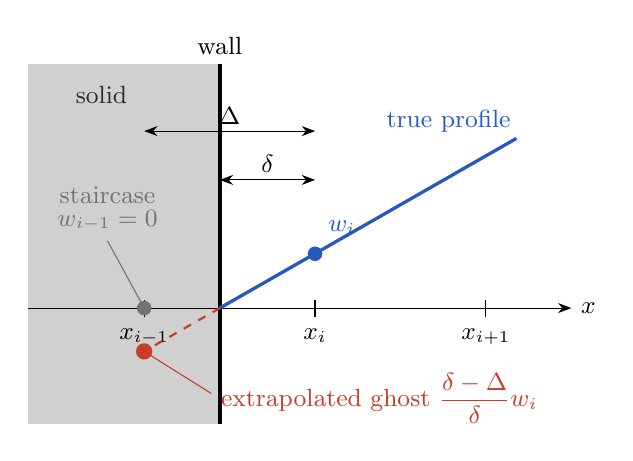
\begin{tikzpicture}[scale=1.55,>=Stealth,font=\small]
  \fill[solidcol,opacity=0.55] (-0.95,-0.95) rectangle (0.62,2.0);
  \draw[very thick] (0.62,-0.95) -- (0.62,2.0);
  \node[above] at (0.62,2.0) {wall};
  \node[solidcol!25!black] at (-0.35,1.75) {solid};
  \draw[->] (-0.95,0) -- (3.5,0) node[right] {$x$};
  \foreach \x/\lab in {0/{i-1},1.4/{i},2.8/{i+1}}
     \draw (\x,0.07) -- (\x,-0.07) node[below=1pt] {$x_{\lab}$};
  % true solution (linear near the wall)
  \draw[very thick,cold] (0.62,0) -- (3.05,1.39);
  \node[cold,above left=-2pt] at (3.05,1.39) {true profile};
  \fill[cold] (1.4,0.445) circle (1.7pt);
  \node[cold] at (1.62,0.66) {$w_i$};
  % staircase ghost
  \fill[black!55] (0,0) circle (1.7pt);
  \draw[black!55,thin] (0,0) -- (-0.30,0.55);
  \node[black!55,align=center,anchor=south] at (-0.30,0.55)
     {staircase\\[-1mm] $w_{i-1}=0$};
  % extrapolated ghost
  \fill[hot] (0,-0.355) circle (1.9pt);
  \draw[hot,dashed,thick] (0.62,0) -- (0,-0.355);
  \draw[hot,thin] (0,-0.355) -- (0.55,-0.70);
  \node[hot,anchor=west] at (0.55,-0.74)
     {extrapolated ghost $\displaystyle\frac{\delta-\Delta}{\delta}w_i$};
  % distances, well above the profile
  \draw[<->] (0.62,1.05) -- node[above=-1pt]{$\delta$} (1.4,1.05);
  \draw[<->] (0,1.45) -- node[above=-1pt]{$\Delta$} (1.4,1.45);
\end{tikzpicture}
\caption{The Luchini correction on one arm. The staircase ghost value (grey)
places the wall at $x_{i-1}$ and is first-order; the linear extrapolation
through $(x_i,w_i)$ and the true wall (red) restores second order. The
extrapolated value is never stored: substituting it into the Laplacian changes
only the centre weight, by $\lambda$ of Eq.~\eqref{eq:lambda}.}
\label{fig:luchini}
\end{figure}

\paragraph{Why this cannot express CHT.}
Equation~\eqref{eq:luchini-ghost} needs the wall value to be \emph{known}. In
CHT the interface temperature $T_\Gamma$ is an unknown determined by the flux
balance with the solid. Reference~\cite{luchini2025} is explicit about the
limitation (their \S3.4): Neumann-type conditions are supported only in
configurations \emph{where the immersed boundary is not involved}. A conjugate
interface is neither Dirichlet nor Neumann --- it is a transmission condition.

\subsection{EJIIM: jump-corrected differences}
\label{sec:ejiim}

Reference~\cite{ejiim2000} keeps the \emph{standard} stencil everywhere and
corrects it with the jumps of the solution and its derivatives. Their Lemma~3,
for an interface at $\alpha\in[x_j,x_{j+1})$ with $h^-=x_j-\alpha$,
$h^+=x_{j+1}-\alpha$, reads
\begin{equation}
  u_{xx}(x_j) \approx \frac{u(x_{j+1})-2u(x_j)+u(x_{j-1})}{h^2}
    - \frac{1}{h^{2}}\sum_{m=0}^{3}\frac{(h^{+})^{m}}{m!}\jump{u^{(m)}} .
  \label{eq:ejiim-lemma3}
\end{equation}
For the composite-material problem $\grad\!\cdot(\beta\grad u)=f$ (their
Problem~(c)) with perfect contact, the jumps are, in interface-local
coordinates $(\xi,\eta)$ (normal, tangential) --- their Eq.~(42) with
$w=\tilde v=0$:
\begin{equation}
  \jump{u}=0,\quad
  \jump{u_\eta}=0,\quad
  \jump{u_\xi}=(\rho-1)\,u^-_\xi,\quad
  \jump{u_{\eta\eta}}=\theta'\jump{u_\xi},\quad
  \rho=\frac{\beta^-}{\beta^+},
  \label{eq:ejiim-jumps}
\end{equation}
plus second-order jumps obtained from the divided equation. The Cartesian jumps
needed by \eqref{eq:ejiim-lemma3} follow by the rotation of their \S5. Two
features matter here:
\begin{enumerate}
\item $\jump{u_\xi}$ depends on the solution, so it is carried as an
      \emph{explicit extra unknown} and the augmented system is solved by a
      Schur complement plus GMRES (their \S6.3):
      $\left(I+D^{T}\Delta_h^{-1}\Psi\right)C = F_2-D^{T}\Delta_h^{-1}F_1$.
\item Their Remark~24: it suffices to have truncation error $O(h)$ \emph{near
      the interface} and $O(h^2)$ elsewhere to obtain $O(h^2)$ convergence in
      the max norm. This licenses dropping the second-derivative jump terms in
      a first implementation.
\end{enumerate}

\paragraph{Why this cannot be adopted verbatim.}
The augmented system, the GMRES solve, and the one-sided six-point
interpolation operators $P_S^{-1}R_S$ (reaching two cells) are incompatible with
an explicit RK3 march, a 26-neighbour single-layer halo, block decomposition
with $2\!:\!1$ refinement, and GPU offload.

\subsection{Cipelli et al.: the corner correction (COCO)}
\label{sec:coco-intro}

Reference~\cite{cipelli2025} sharpens \cite{luchini2025} exactly where the
geometry is singular. Their observation is that the linear near-wall profile
behind Eq.~\eqref{eq:luchini-ghost} is merely the \emph{simplest} local
solution; near a sharp corner the correct local behaviour is the steady Stokes
solution of the same wedge (for a component decoupled from the pressure
gradient, a Laplace solution, e.g.\ $u_S=A\,r^{m}\cos m\theta$ with
$m=\pi/2\varphi_w$ for a wedge of half-opening $\varphi_w$). They therefore
require the discrete solution to match a \emph{rescaled} local analytic
solution,
\begin{equation}
  u_e(\boldsymbol{x}) = \frac{u_S(\boldsymbol{x})}{u_S(\boldsymbol{x}_0)}\;
                        u_\alpha(i,j,k),
  \label{eq:coco-rescale}
\end{equation}
which yields the correction coefficient (their Eq.~11)
\begin{equation}
  \lambda_\alpha=\sum_{l=1}^{3}\left[
     d^{(2)}_l(0)
   + d^{(2)}_l(-1)\frac{u_S(\boldsymbol{x}_0-\Delta\boldsymbol{x}_l)}{u_S(\boldsymbol{x}_0)}
   + d^{(2)}_l(+1)\frac{u_S(\boldsymbol{x}_0+\Delta\boldsymbol{x}_l)}{u_S(\boldsymbol{x}_0)}
     \right] - (\text{pressure terms}).
  \label{eq:coco-lambda}
\end{equation}
Three properties matter for what follows.
\begin{enumerate}
\item[(i)] $u_S$ enters only through \textbf{ratios}, so its amplitude $A$ is
      irrelevant and $\lambda_\alpha$ is a pure \emph{geometric} number,
      precomputed once before the run --- the same storage and the same
      implicit treatment \eqref{eq:luchini-B} as the plain IBM coefficient.
\item[(ii)] The correction is $-\mathcal{L}_\Delta(u_e)$ where $\mathcal{L}$ is
      the continuous Stokes operator and $\mathcal{L}(u_e)=0$ \emph{exactly}
      (their Eq.~14). It therefore vanishes automatically wherever the discrete
      operator is accurate, which is what allows it to be applied at points
      \emph{not} adjacent to the wall --- in practice within a radius
      $\approx2\Delta$ of the tip.
\item[(iii)] For a flat wall $u_S$ is the Couette profile and
      \eqref{eq:coco-lambda} reduces \emph{exactly} to Luchini's $\lambda$,
      Eq.~\eqref{eq:lambda}.
\end{enumerate}
Property (iii) is the invitation taken up in Sec.~\ref{sec:coco}: a smooth
interface is the $180^\circ$ member of the same family, and a conjugate
interface is the two-material member.

%======================================================================
\section{The bridge: explicitness collapses the augmented system}
%======================================================================

The scalars in \textsc{mobydiff} are advanced \emph{fully explicitly}
(\code{scalar\_transport}, RK3 low-storage, no linear solve --- unlike the
pressure). At the start of each substage the field is known everywhere, in the
solid as well as in the fluid. Therefore
\begin{center}
\emph{every one-sided limit appearing in the EJIIM jump conditions
      \eqref{eq:ejiim-jumps} is computable from the current field.}
\end{center}
EJIIM's ``unknown jump'' is unknown only because the elliptic problem is solved
implicitly. For us it is data. The augmented system, the Schur complement and
GMRES all collapse to a \emph{local, explicit evaluation at cut faces}. This is
the single structural simplification that makes the scheme affordable, and it is
available precisely because the scalar --- unlike the pressure --- needs no
global solve.

What remains from \cite{luchini2025} is then the \emph{shape} of the treatment:
correct the diffusive operator only, keep the correction local, and eliminate
the interface unknown analytically rather than storing it.

%======================================================================
\section{Derivation of the cut-face flux}
\label{sec:derivation}
%======================================================================

\subsection{Setup}

Refer again to Fig.~\ref{fig:geometry}. Let
\begin{equation}
  a=\nn\cdot\ed,
  \qquad
  \partial_nT = \nn\cdot\grad T,
  \qquad
  \grad_t T = \grad T-\nn\,\partial_n T .
\end{equation}
Because $\jump{T}_\Gamma=0$ holds along all of $\Gamma$, the \emph{tangential}
gradient is continuous:
\begin{equation}
  \grad_tT^{-}\big|_P = \grad_tT^{+}\big|_P \equiv \grad_tT\big|_P .
  \label{eq:tang-cont}
\end{equation}
Define the scalar
\begin{equation}
  s_t \;\equiv\; \ed\cdot\grad_tT\big|_P
     \;=\; \ed\cdot\grad T - a\,\partial_nT ,
  \label{eq:st}
\end{equation}
the part of the coordinate-direction derivative that is \emph{not} carried by
the normal. By \eqref{eq:tang-cont}, $s_t$ may be evaluated from either side.
Finally, the flux-continuity condition \eqref{eq:interface} defines the single
continuous quantity
\begin{equation}
  q_n \;\equiv\; k_L\,\partial_nT^{-}\big|_P \;=\; k_R\,\partial_nT^{+}\big|_P .
  \label{eq:qn}
\end{equation}

\subsection{Elimination of the interface temperature}

Expand $T$ about $P$ on each side, along $\ed$:
\begin{align}
  T_L &= T_\Gamma - \delta_L\left(\ed\cdot\grad T^{-}\right)+O(h^2)
       = T_\Gamma - \delta_L\left(\frac{a\,q_n}{k_L}+s_t\right)+O(h^2),
       \label{eq:TL}\\
  T_R &= T_\Gamma + \delta_R\left(\ed\cdot\grad T^{+}\right)+O(h^2)
       = T_\Gamma + \delta_R\left(\frac{a\,q_n}{k_R}+s_t\right)+O(h^2),
       \label{eq:TR}
\end{align}
where \eqref{eq:st} and \eqref{eq:qn} have been used on each side separately.
Subtracting, $T_\Gamma$ cancels:
\begin{equation}
  \boxed{\;
  T_R-T_L = a\,q_n\,\Rser + h_d\,s_t + O(h^2),
  \qquad
  \Rser \equiv \frac{\delta_L}{k_L}+\frac{\delta_R}{k_R} \; }
  \label{eq:master}
\end{equation}
The quantity $\Rser$ is the \emph{series thermal resistance} of the two
sub-segments, exactly as in the electrical analogue of
Fig.~\ref{fig:resistance}. Solving for the normal flux,
\begin{equation}
  a\,q_n = \frac{T_R-T_L-h_d\,s_t}{\Rser}.
  \label{eq:qn-solved}
\end{equation}

\begin{figure}[htbp]
\centering
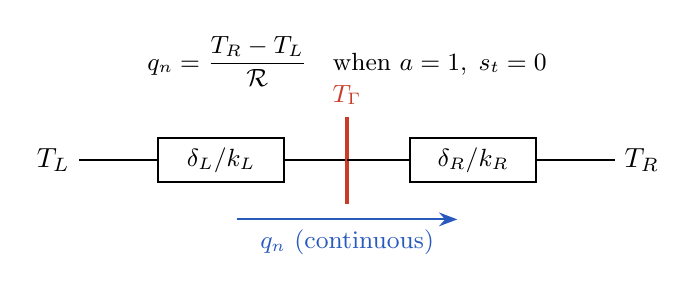
\begin{tikzpicture}[scale=1.0,>=Stealth]
  \draw[thick] (0,0) -- (1.0,0);
  \draw[thick] (1.0,-0.28) rectangle (2.6,0.28);
  \node at (1.8,0) {\small $\delta_L/k_L$};
  \draw[thick] (2.6,0) -- (3.4,0);
  \draw[very thick,hot] (3.4,-0.55) -- (3.4,0.55);
  \node[hot,above] at (3.4,0.58) {\small $T_\Gamma$};
  \draw[thick] (3.4,0) -- (4.2,0);
  \draw[thick] (4.2,-0.28) rectangle (5.8,0.28);
  \node at (5.0,0) {\small $\delta_R/k_R$};
  \draw[thick] (5.8,0) -- (6.8,0);
  \node[left]  at (0,0) {$T_L$};
  \node[right] at (6.8,0) {$T_R$};
  \draw[->,thick,cold] (2.0,-0.75) -- (4.8,-0.75)
      node[midway,below,font=\small,cold]{$q_n$ (continuous)};
  \node[font=\small] at (3.4,1.25)
     {$\displaystyle q_n=\frac{T_R-T_L}{\Rser}\quad\text{when }a=1,\;s_t=0$};
\end{tikzpicture}
\caption{Electrical analogue of Eq.~\eqref{eq:master}. The two sub-segments are
resistances in series; the interface temperature $T_\Gamma$ is the internal node
and is eliminated. The resistance $\Rser\ge h_d/\max(k_L,k_R)$ is bounded away
from zero for \emph{any} cut position --- the origin of the non-stiffness result
of Sec.~\ref{sec:stability}.}
\label{fig:resistance}
\end{figure}

\subsection{The flux the discretisation needs}

The finite-volume/finite-difference kernel needs the diffusive flux component in
the coordinate direction, at the cell face. In the solver's sign convention
(\code{scalar\_transport\_kernel} forms \code{fe}, \code{fw} as
$D_{\text{face}}(T_R-T_L)/\Delta$ and then $(\code{fe}-\code{fw})\,d1x$), the
required quantity is
\begin{equation}
  F \;\equiv\; k\,\ed\cdot\grad T\Big|_{\text{face}} .
\end{equation}
The face midpoint lies on one definite side; call the local conductivity there
$k_{\text{loc}}$ (that of the side containing the face midpoint). Using
\eqref{eq:st} and \eqref{eq:qn} on that side,
\begin{equation}
  F = k_{\text{loc}}\left(a\,\partial_nT + s_t\right)
    = a\,q_n + k_{\text{loc}}\,s_t ,
\end{equation}
and substituting \eqref{eq:qn-solved} gives the central result:
\begin{equation}
  \boxed{\;
  F \;=\; \frac{T_R-T_L}{\Rser}
        \;+\; s_t\left(k_{\text{loc}}-\frac{h_d}{\Rser}\right)
  \; }
  \label{eq:main}
\end{equation}

\subsection{Structure of the result}

Equation~\eqref{eq:main} deserves to be read slowly.

\begin{description}
\item[The obliquity $a$ has cancelled.] It appears nowhere in
      \eqref{eq:main}. The series-resistance term is the correct leading
      behaviour for \emph{any} interface orientation; the orientation enters only
      through $\Rser$ (via $\delta_L,\delta_R$) and through the definition of
      $s_t$.
\item[The first term is an exact resummation.] Expanding
      $1/\Rser$ for small conductivity contrast reproduces the linearised
      EJIIM correction $\propto\jump{u_\xi}=(\rho-1)u^-_\xi$ of
      Eq.~\eqref{eq:ejiim-jumps}; but the closed form stays bounded for
      \emph{all} contrasts, including $k_R/k_L\to0$ and $\to\infty$, whereas the
      linearised correction does not. This is why the resistance form, and not
      the truncated jump series, is the right backbone.
\item[The correction needs only continuous data.] $s_t$ is a tangential
      gradient, continuous by \eqref{eq:tang-cont}. The \emph{discontinuous}
      normal derivative has been resummed exactly into $\Rser$. The
      ill-conditioned one-sided reconstruction that makes EJIIM expensive at high
      contrast is therefore not needed for the piece we evaluate explicitly.
\item[It is a flux.] Written into the face-flux form, \eqref{eq:main} enters the
      two adjacent cell balances with opposite signs, so
      $\sum_{\text{cells}}\rho c\,T\,\Delta V$ is conserved to round-off
      \emph{regardless} of how accurate $s_t$ is. Accuracy and conservation are
      decoupled.
\end{description}

\subsection{Limits and consistency checks}
\label{sec:limits}

\begin{table}[htbp]
\centering
\caption{Equation~\eqref{eq:main} in its limits. Every check is analytic.}
\label{tab:limits}
\begin{tabular}{@{}lll@{}}
\toprule
Limit & $\Rser$, $h_d/\Rser$ & $F$ \\
\midrule
Homogeneous, $k_R=k_L=k$
  & $h_d/k$, \; $k$
  & $k\,(T_R-T_L)/h_d$ \quad(correction vanishes)\\
Grid-aligned, $\nn\parallel\ed$
  & ---
  & $(T_R-T_L)/\Rser$ \quad($s_t=0$)\\
Isothermal body, $k_R\to\infty$
  & $\delta_L/k_L$
  & $k_L\,(T_\text{body}-T_L)/\delta_L$ \quad$=$ Luchini $\lambda$ \\
Adiabatic body, $k_R\to0$
  & $\infty$, \; $0$
  & $k_L\,s_t$ \quad(pure tangential conduction)\\
\bottomrule
\end{tabular}
\end{table}

The third row deserves a line of algebra, because it is the exact bridge to
\cite{luchini2025}. With $k_R\to\infty$ the solid is isothermal at
$T_{\text{body}}$ and, since $T\equiv T_{\text{body}}$ on $\Gamma$, we also have
$\grad_tT=0$, hence $s_t=0$ identically. Then
$F_w=k_L(T_{\text{body}}-T_L)/\delta_L$. For $T_{\text{body}}=0$ on a uniform
mesh the resulting contribution to the cell balance is
\begin{equation}
  -\frac{F_w}{\Delta} = -\frac{k_L T_L}{\delta\,\Delta}
  \quad\text{versus the unmodified}\quad
  -\frac{k_L T_L}{\Delta^{2}},
  \qquad\text{difference }= -k_L\frac{\Delta-\delta}{\delta\Delta^{2}}\,T_L,
\end{equation}
which is exactly $-\lambda T_L$ of Eq.~\eqref{eq:lambda}, i.e.\ exactly the
coefficient \code{ibm.f90} already stores. \textbf{The Luchini correction is the
$k_s\to\infty$ limit of Eq.~\eqref{eq:main}, algebraically identical, including
the code's $\big((d_0-d)/d\big)/d_0^{2}$ form.} The adiabatic mode is its
$k_s\to0$ limit. One implementation therefore delivers three body thermal
modes.

\subsection{Why Luchini needs no tangential term and CHT does}
\label{sec:whytangential}

This is the conceptual heart of the matter and is illustrated in
Fig.~\ref{fig:tangential}. For a \emph{Dirichlet} boundary the boundary value is
prescribed along $\Gamma$, so
\begin{equation}
  T\big|_\Gamma = T_{\text{body}} = \text{const}
  \quad\Longrightarrow\quad
  \grad_tT\big|_\Gamma \equiv 0
  \quad\Longrightarrow\quad
  s_t \equiv 0 .
\end{equation}
The same holds for the no-slip velocity condition $\boldsymbol{u}|_\Gamma=0$.
A purely dimension-split, one-dimensional correction is then \emph{exact in
structure}, and \cite{luchini2025} legitimately attains second order without any
rotation, tangential term, or normal reconstruction --- their entire correction
being $\lambda$.

At a \emph{conjugate} interface the interface temperature $T_\Gamma(\boldsymbol{x})$
\emph{varies along $\Gamma$}: it is an outcome, not a datum. Hence
$\grad_tT\neq0$, $s_t\neq0$, and the term
$s_t\,(k_{\text{loc}}-h_d/\Rser)$ in \eqref{eq:main} is $O(1)$ --- it does not
vanish as $h\to0$. Dropping it (i.e.\ using distance-weighted harmonic averaging
alone, the ``obvious'' scheme) leaves an $O(1)$ error in the local flux at every
obliquely cut face, proportional to the conductivity contrast. This is the
classic and well-documented failure of naive harmonic averaging on non-aligned
interfaces, and it is exactly the deficiency that the EJIIM rotation machinery
repairs.

The rigorous form of this statement is a \emph{parameter count}, deferred to
Sec.~\ref{sec:counting}: the local conjugate solution carries three free
parameters against the Dirichlet problem's one, while a cut arm supplies only
two equations. One parameter must therefore always come from a transverse
stencil --- so no arm-local scheme, harmonic averaging included, can be second
order on an oblique conjugate interface.

\begin{figure}[htbp]
\centering
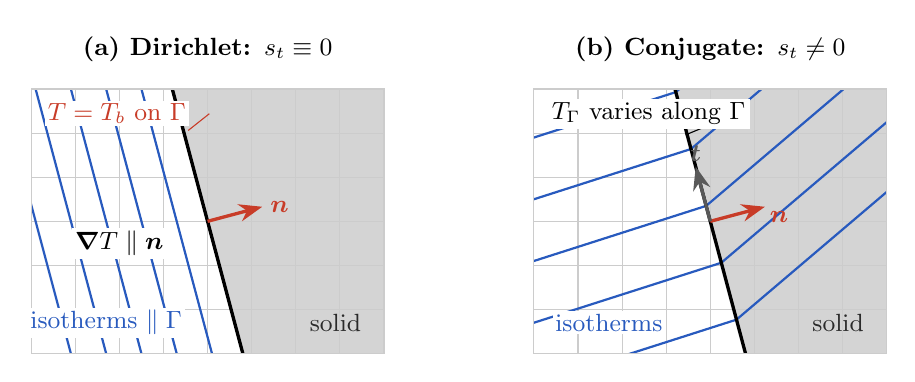
\begin{tikzpicture}[scale=1.12,>=Stealth,font=\small]
  % ---------------- (a) Dirichlet ----------------
  \begin{scope}
    \node[font=\bfseries\small] at (2.0,3.45) {(a) Dirichlet: $s_t\equiv0$};
    \begin{scope}
      \clip (0,0) rectangle (4,3);
      \fill[solidcol,opacity=0.5] (2.4,0) -- (4,0) -- (4,3) -- (1.6,3) -- cycle;
      \draw[gray!40] (0,0) grid[step=0.5] (4,3);
      % isotherms parallel to the interface, fluid side only
      \begin{scope}
        \clip (0,0) -- (2.4,0) -- (1.6,3) -- (0,3) -- cycle;
        \foreach \s in {0.35,0.75,1.15,1.55,1.95}
          \draw[cold,thick] ({2.4-\s},0) -- ({1.6-\s},3);
      \end{scope}
      \draw[very thick] (2.4,0) -- (1.6,3);
    \end{scope}
    \draw[gray!40] (0,0) rectangle (4,3);
    \node[cold,fill=white,inner sep=1pt] at (0.85,0.35) {isotherms $\parallel\Gamma$};
    \draw[->,very thick,hot] (2.0,1.5) -- ++(0.62,0.165) node[right=-1pt]{$\nn$};
    \draw[hot,thin] (1.78,2.53) -- (2.02,2.72);
    \node[hot,anchor=west,fill=white,inner sep=1pt] at (0.15,2.72) {$T=T_b$ on $\Gamma$};
    \node[fill=white,inner sep=1pt] at (1.00,1.25) {$\grad T\parallel\nn$};
    \node[solidcol!25!black] at (3.45,0.35) {solid};
  \end{scope}
  % ---------------- (b) Conjugate ----------------
  \begin{scope}[xshift=5.7cm]
    \node[font=\bfseries\small] at (2.0,3.45) {(b) Conjugate: $s_t\neq0$};
    \begin{scope}
      \clip (0,0) rectangle (4,3);
      \fill[solidcol,opacity=0.5] (2.4,0) -- (4,0) -- (4,3) -- (1.6,3) -- cycle;
      \draw[gray!40] (0,0) grid[step=0.5] (4,3);
      % isotherms oblique to the interface, KINKED across it (k_s > k_f)
      \foreach \yz in {-0.35,0.35,1.05,1.75,2.45} {
        \pgfmathsetmacro{\ycut}{(\yz + 2.4*0.32)/(1+0.2667*0.32)}
        \pgfmathsetmacro{\xcut}{2.4-0.2667*\ycut}
        \draw[cold,thick] (0,\yz) -- (\xcut,\ycut) -- (4,{\ycut+0.85*(4-\xcut)});
      }
      \draw[very thick] (2.4,0) -- (1.6,3);
    \end{scope}
    \draw[gray!40] (0,0) rectangle (4,3);
    \draw[->,very thick,hot]   (2.0,1.5) -- ++(0.62,0.165) node[below right=-3pt]{$\nn$};
    \draw[->,very thick,black!65] (2.0,1.5) -- ++(-0.165,0.62) node[above=-2pt]{$\boldsymbol{t}$};
    \node[cold,fill=white,inner sep=1pt] at (0.85,0.35) {isotherms};
    \draw[thin] (1.72,2.48) -- (2.30,2.72);
    \node[anchor=west,fill=white,inner sep=1.5pt] at (0.15,2.72)
       {$T_\Gamma$ varies along $\Gamma$};
    \node[solidcol!25!black] at (3.45,0.35) {solid};
  \end{scope}
\end{tikzpicture}
\caption{(a) With a prescribed body temperature the isotherms meet $\Gamma$
parallel to it, $\grad T$ is purely normal, and the tangential term is
identically zero --- a dimension-split correction suffices, which is why
\cite{luchini2025} needs nothing more. (b) At a conjugate interface the
interface temperature varies along $\Gamma$; $\grad T$ has a tangential
component that a dimension-split flux misattributes to the normal direction,
producing an $O(1)$ flux error proportional to the conductivity contrast.}
\label{fig:tangential}
\end{figure}

\subsection{Accuracy}
\label{sec:accuracy}

The expansions \eqref{eq:TL}--\eqref{eq:TR} were truncated after the linear
term. The neglected contributions are
$\tfrac12\delta_R^{2}(\ed\!\cdot\!\grad)^2T^{+}
 -\tfrac12\delta_L^{2}(\ed\!\cdot\!\grad)^2T^{-}$
in $T_R-T_L$, hence an $O(h)\,k\,T''$ error in the flux \eqref{eq:main}. Two
observations:
\begin{enumerate}
\item In the homogeneous case this ``error'' is not an error at all: since
      $\Rser=h_d/k$, the two terms combine into
      $(\delta_R-\delta_L)/2 \cdot T''$, which is precisely the shift from the
      interface point $P$ to the \emph{face midpoint}. The two-point flux is then
      second-order accurate at the face midpoint, as it must be --- and
      Eq.~\eqref{eq:main} reduces identically to the existing kernel.
\item With a conductivity jump the cancellation is only partial, and a residual
      $O(h)$ flux error survives at cut faces. Because the scheme is a discrete
      divergence of a consistent flux, this yields $O(h)$ truncation error on the
      $O(h)$-measure interface band and $O(h^2)$ elsewhere --- exactly the
      regime that \cite{ejiim2000}, Remark~24, certifies as giving $O(h^2)$
      convergence in the max norm.
\end{enumerate}
Consequently the second-derivative jump terms of \eqref{eq:ejiim-jumps} are
\emph{optional}. They are the natural first escalation if the measured
convergence order falls short; the unsteady contribution to $\jump{u_{\xi\xi}}$
is $\jump{f/\beta}=\partial_tT\left(\alpha_s^{-1}-\alpha_f^{-1}\right)$, and it
vanishes at the interface in the steady case (the convective part of $f$
vanishes there because $\boldsymbol{u}|_\Gamma=0$ for a stationary body).

\subsection{Contact resistance}
\label{sec:contact}

For imperfect contact, $\jump{T}_\Gamma = R_c\,q_n$, Eq.~\eqref{eq:TR} acquires
$T_\Gamma^{+}=T_\Gamma^{-}+R_c q_n$ and the derivation goes through unchanged
with
\begin{equation}
  \Rser \;\longrightarrow\; \frac{\delta_L}{k_L}+R_c+\frac{\delta_R}{k_R}.
\end{equation}
Nothing else changes; note that $R_c>0$ makes the tangential gradient
discontinuous at $O(R_c\,\partial_t q_n)$, which is beyond the order retained here.

%======================================================================
\section{The COCO route: the same scheme from a local-solution viewpoint}
\label{sec:coco}
%======================================================================

Section~\ref{sec:derivation} obtained \eqref{eq:main} by Taylor expansion around
the cut point. The corner-correction idea of \cite{cipelli2025}
(Sec.~\ref{sec:coco-intro}) reaches the same place by a shorter and more
physical route, and --- unlike the Taylor argument --- it keeps going where the
interface stops being smooth.

\subsection{Two complementary wedges}
\label{sec:wedges}

Apply the COCO recipe to conduction. The dominant local operator is the Laplace
operator on each side, subject to the transmission conditions
\eqref{eq:interface}. For a \emph{locally flat} interface the two media occupy
two complementary $180^\circ$ wedges (Fig.~\ref{fig:wedges}a), and the local
solution of the transmission problem is
\begin{equation}
  T(\boldsymbol{x}) \;=\; T_\Gamma
    \;+\; a_t\,\underbrace{(\boldsymbol{x}\!-\!P)\cdot\boldsymbol{t}}_{\text{tangential}}
    \;+\; \frac{q_n}{k^{\pm}}\,
          \underbrace{(\boldsymbol{x}\!-\!P)\cdot\nn}_{\text{normal}}
    \;+\;O(r^{2}),
  \label{eq:localmodel}
\end{equation}
with the SAME $q_n$ on both sides --- which is precisely the statement that the
wall-normal derivatives of the two complementary wedge solutions match, weighted
by their conductivities. The tangential slope $a_t$ is common to both sides
because $\jump{T}=0$ along $\Gamma$. Evaluating \eqref{eq:localmodel} at the two
cell centres and subtracting eliminates $T_\Gamma$ and returns
\begin{equation}
  T_R-T_L = a\,q_n\Rser + h_d\,a_t ,
\end{equation}
which is Eq.~\eqref{eq:master} identically, with $a_t\equiv s_t$. \textbf{The
COCO construction with $180^\circ/180^\circ$ wedges IS the series-resistance
scheme}, obtained without a single Taylor expansion. Two by-products of the
agreement are worth recording:
\begin{itemize}
\item It is an \emph{independent derivation} of \eqref{eq:main}: two different
      routes, no free constants, same formula.
\item It exposes the relationship between the two source methods:
      \textbf{COCO $\equiv$ EJIIM with the jump data supplied by an analytic
      local solution} instead of by differentiating the jump conditions. Both
      are deferred corrections built from a locally exact solution; they differ
      only in where the local solution comes from.
\end{itemize}
Approximating a smooth surface by locally flat pieces at the local inclination
--- ``piecewise $180^\circ$ wedges'' --- is legitimate at the order required:
curvature enters the next term, i.e.\ the $O(h)$ flux residual on the interface
band that Sec.~\ref{sec:accuracy} already accounts for. One refinement worth
adopting: build \emph{one} local plane per cut cell (or per cut face), not one
per arm, so that the six arms of a cell do not each carry a slightly different
interface plane.

\begin{figure}[htbp]
\centering
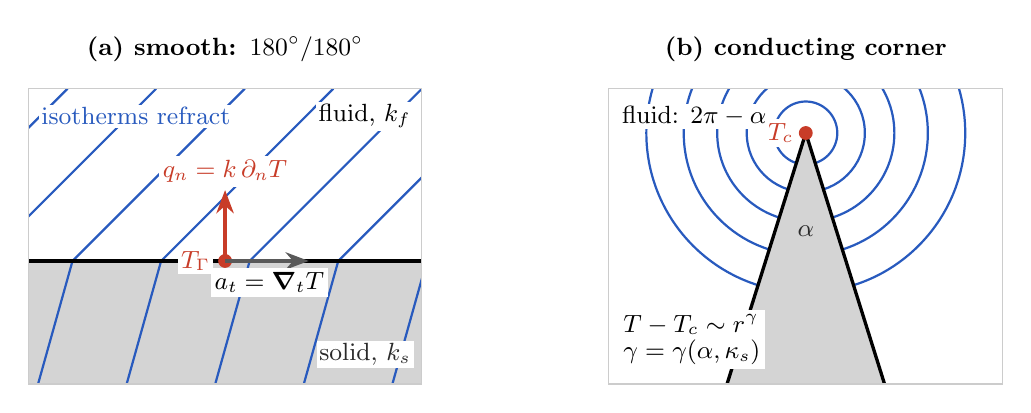
\begin{tikzpicture}[scale=1.25,>=Stealth,font=\small]
  % ---------------- (a) two complementary 180 degree wedges ------------
  \begin{scope}
    \node[font=\bfseries\small] at (2.0,3.40) {(a) smooth: $180^\circ/180^\circ$};
    \begin{scope}
      \clip (0,0) rectangle (4,3);
      \fill[solidcol,opacity=0.5] (0,0) rectangle (4,1.25);
      % isotherms refract at the interface: tangential slope continuous,
      % k * normal derivative continuous  (fluid side much shallower)
      \foreach \xz in {-2.6,-1.7,-0.8,0.1,1.0,1.9,2.8,3.7}
        \draw[cold,thick] (\xz,0) -- ({\xz+0.35},1.25) -- ({\xz+0.35+1.75},3);
      \draw[very thick] (0,1.25) -- (4,1.25);
    \end{scope}
    \draw[gray!40] (0,0) rectangle (4,3);
    \node[anchor=east,fill=white,inner sep=1pt] at (3.92,2.72) {fluid, $k_f$};
    \node[solidcol!25!black,anchor=east,fill=white,inner sep=1pt]
        at (3.92,0.30) {solid, $k_s$};
    \node[cold,anchor=west,fill=white,inner sep=1pt] at (0.10,2.72)
        {isotherms refract};
    \fill[hot] (2.0,1.25) circle (2.0pt);
    \node[hot,anchor=east,fill=white,inner sep=1pt] at (1.88,1.25) {$T_\Gamma$};
    \draw[->,very thick,hot] (2.0,1.25) -- ++(0,0.72);
    \node[hot,anchor=south,fill=white,inner sep=1.5pt] at (2.0,2.00)
        {$q_n=k\,\partial_nT$};
    \draw[->,very thick,black!65] (2.0,1.25) -- ++(0.85,0);
    \node[anchor=north,fill=white,inner sep=1.5pt] at (2.45,1.18)
        {$a_t=\grad_tT$};
  \end{scope}
  % ---------------- (b) conducting sharp corner ------------------------
  \begin{scope}[xshift=5.9cm]
    \node[font=\bfseries\small] at (2.0,3.40) {(b) conducting corner};
    \begin{scope}
      \clip (0,0) rectangle (4,3);
      % isotherms wrapping the tip, then the solid wedge painted OVER them
      % (an opaque fill is the simple stand-in for clipping to the fluid)
      \foreach \rr in {0.32,0.60,0.90,1.24,1.62}
        \draw[cold,thick] (2.0,2.55) circle (\rr);
      \fill[solidcol!50!white] (2.0,2.55) -- (1.20,0) -- (2.80,0) -- cycle;
      \draw[very thick] (1.20,0) -- (2.0,2.55) -- (2.80,0);
    \end{scope}
    \draw[gray!40] (0,0) rectangle (4,3);
    \fill[hot] (2.0,2.55) circle (2.0pt);
    \node[hot,anchor=east,fill=white,inner sep=1.5pt] at (1.92,2.55) {$T_c$};
    \node[solidcol!25!black] at (2.0,1.55) {$\alpha$};
    \node[anchor=west,fill=white,inner sep=1pt] at (0.10,2.72) {fluid: $2\pi-\alpha$};
    \node[anchor=west,align=left,fill=white,inner sep=1.5pt] at (0.10,0.45)
        {$T-T_c\sim r^{\gamma}$\\[-0.5mm] $\gamma=\gamma(\alpha,\kappa_s)$};
  \end{scope}
\end{tikzpicture}
\caption{(a) A smooth conjugate interface is the $180^\circ/180^\circ$ member of
the wedge family. The local solution \eqref{eq:localmodel} has three free
parameters --- $T_\Gamma$, the tangential slope $a_t$, the normal flux $q_n$ ---
and matching the two complementary normal derivatives is exactly the series
resistance. Isotherms refract at $\Gamma$: the tangential gradient is
continuous, $k\,\partial_nT$ is continuous, so the normal gradient kinks.
(b) A conducting sharp corner: the wedges are $\alpha$ (solid) and
$2\pi-\alpha$ (fluid), the leading exponent $\gamma$ solves a transcendental
condition depending on the angle \emph{and} the conductivity ratio, and the
locally flat model of (a) fails at leading order.}
\label{fig:wedges}
\end{figure}

\subsection{Parameter counting: when a single $\lambda$ exists}
\label{sec:counting}

The reason COCO's coefficient \eqref{eq:coco-lambda} is a pure geometric number
is that the no-slip condition pins the local solution up to \emph{one} scale:
$u_S$ is fixed as a shape, the amplitude cancels in the ratios, and the
correction can be written as $\lambda$ times the single nodal value. Count the
free parameters of the local model in the two problems:

\begin{table}[htbp]
\centering
\caption{Free parameters of the local solution, and what the discretisation can
supply. ``Arm'' means the two cell values $T_L,T_R$ straddling the interface.}
\label{tab:counting}
\begin{tabular}{@{}lccc@{}}
\toprule
problem & local model & free parameters & equations from one arm \\
\midrule
velocity, no slip (\cite{luchini2025,cipelli2025})
  & $A\,u_S(\boldsymbol{x})$, $u_S|_\Gamma=0$
  & \textbf{1} & 1 \\
conjugate interface (this note)
  & Eq.~\eqref{eq:localmodel}
  & \textbf{3} ($T_\Gamma$, $a_t$, $q_n$) & 2 \\
\bottomrule
\end{tabular}
\end{table}

Two consequences, both structural:
\begin{enumerate}
\item \textbf{No single precomputed $\lambda$ can exist for CHT.} The
      correction cannot be proportional to one nodal value; it must be linear
      in a locally \emph{reconstructed} state. COCO's ratio form is available
      if and only if the boundary condition pins the local solution up to one
      scale, i.e.\ iff it is homogeneous-Dirichlet-like. A conjugate interface
      never is --- and the one limit in which it degenerates,
      $\kappa_s\to\infty$ with a prescribed body temperature, is precisely the
      Dirichlet case of \cite{luchini2025}.
\item \textbf{Transverse data is mandatory, always.} One arm gives two
      equations for three parameters. The missing one is $a_t\equiv s_t$, which
      is exactly why Sec.~\ref{sec:derivation} had to import it from a wider
      stencil, and it settles the question raised in
      Sec.~\ref{sec:whytangential} without appealing to measurement: an
      arm-local scheme is one equation short, so it cannot be second order on
      an oblique conjugate interface. The count also fixes the minimum stencil:
      at least one same-side transverse neighbour, i.e.\ the $3^3$ patch of
      Fig.~\ref{fig:stencil}.
\end{enumerate}

\subsection{Two traps when transcribing COCO to CHT}
\label{sec:traps}

\paragraph{(a) The ratio denominator vanishes and changes sign.}
Equation~\eqref{eq:coco-lambda} divides by $u_S(\boldsymbol{x}_0)$. For velocity
$u_S>0$ everywhere in the fluid, so $\lambda>0$ always, and $\lambda\to\infty$
as a node approaches the wall is \emph{benign}: the implicit treatment
\eqref{eq:luchini-B} turns it into the exact Dirichlet condition. The
conduction analogue of $u_S$ is $T-T_\Gamma$, which is \textbf{zero on $\Gamma$
and changes sign across it}. The denominator therefore passes through zero at
points arbitrarily close to the interface on both sides, and the resulting
coefficient is unbounded \emph{and sign-indefinite}; a negative $\lambda$ is
anti-diffusive and implicitness does not cure it. This is the same obstacle as
Sec.~\ref{sec:counting} seen from the algebra, and it has the same resolution:
reconstruct the local state, do not rescale by a nodal value.

\paragraph{(b) A point-anchored correction is not conservative.}
In COCO every grid point uses \emph{its own} rescaled local solution, so the
correction is a \textbf{cell source}, not a flux difference: neighbouring cells
apply mutually inconsistent corrections across the face they share
(Fig.~\ref{fig:anchor}a). For momentum that is an accepted cost. For CHT it
means the interface can create or destroy energy at $O(h)$ per step --- the
error that surfaces as wall-temperature drift over a long conjugate run, and it
would forfeit the conservation gate, which is the sharpest test available.
The fix is to anchor the local model to the \textbf{face}, shared by both
adjacent cells (Fig.~\ref{fig:anchor}b): then $-\mathcal{L}_\Delta(T_e)$ is a
flux difference, it telescopes, and conservation is exact. Doing so returns
\eqref{eq:main} --- the flux form of Sec.~\ref{sec:derivation} is precisely the
face-anchored COCO correction.

\begin{figure}[htbp]
\centering
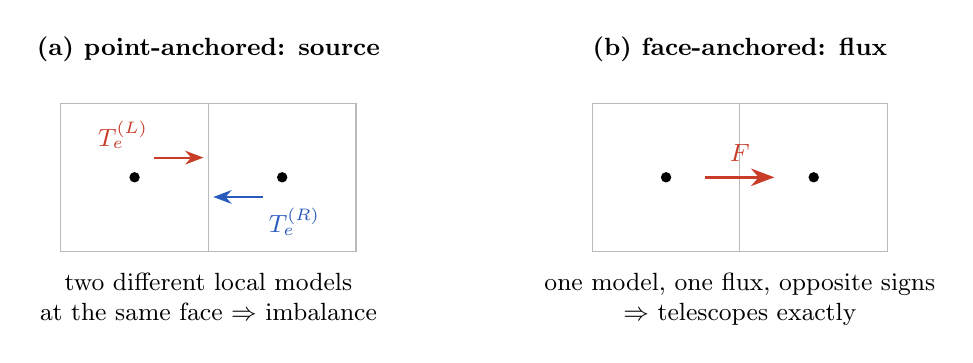
\begin{tikzpicture}[scale=1.25,>=Stealth,font=\small]
  % (a) point anchored
  \begin{scope}
    \node[font=\bfseries\small] at (1.5,2.05) {(a) point-anchored: source};
    \draw[gray!55] (0,0) rectangle (3,1.5);
    \draw[gray!55] (1.5,0) -- (1.5,1.5);
    \fill[black] (0.75,0.75) circle (1.5pt);
    \fill[black] (2.25,0.75) circle (1.5pt);
    \draw[->,thick,hot]  (0.95,0.95) -- (1.45,0.95);
    \draw[->,thick,cold] (2.05,0.55) -- (1.55,0.55);
    \node[hot,anchor=east,inner sep=1pt] at (0.92,1.18) {$T_e^{(L)}$};
    \node[cold,anchor=west,inner sep=1pt] at (2.08,0.30) {$T_e^{(R)}$};
    \node[anchor=north,align=center] at (1.5,-0.12)
       {two different local models\\ at the same face $\Rightarrow$ imbalance};
  \end{scope}
  % (b) face anchored
  \begin{scope}[xshift=5.4cm]
    \node[font=\bfseries\small] at (1.5,2.05) {(b) face-anchored: flux};
    \draw[gray!55] (0,0) rectangle (3,1.5);
    \draw[gray!55] (1.5,0) -- (1.5,1.5);
    \fill[black] (0.75,0.75) circle (1.5pt);
    \fill[black] (2.25,0.75) circle (1.5pt);
    \draw[->,very thick,hot] (1.15,0.75) -- (1.85,0.75);
    \node[hot,anchor=south,inner sep=2pt] at (1.5,0.85) {$F$};
    \node[anchor=north,align=center] at (1.5,-0.12)
       {one model, one flux, opposite signs\\ $\Rightarrow$ telescopes exactly};
  \end{scope}
\end{tikzpicture}
\caption{Why the local model must be attached to the face. (a) COCO's
point-anchored rescaling gives each cell its own local solution, so the two
sides of a face disagree and the correction acts as a cell source. (b) One
model per face yields a single flux entering both balances with opposite signs;
conservation is then exact independently of the model's accuracy.}
\label{fig:anchor}
\end{figure}

\subsection{The genuine extension: conducting sharp corners}
\label{sec:corners}

Everything above says that for a \emph{smooth} interface the COCO route
reproduces \eqref{eq:main}. Its real payoff is the case \eqref{eq:main} does not
cover: a sharp corner carrying a conjugate condition --- a conducting riblet
tip, a fin root, the trailing edge of a conducting body
(Fig.~\ref{fig:wedges}b). There the field is genuinely singular and the locally
flat model fails at leading order, exactly as the linear profile fails for
velocity at a riblet tip.

The construction transfers directly. Replace the no-slip / no-penetration
conditions of \cite{cipelli2025} (their Eq.~21) with
\begin{equation}
  \jump{T}=0,\qquad \jump{k\,\partial_\theta T}=0
  \qquad\text{on both wedge faces,}
\end{equation}
and solve the same kind of homogeneous linear system $M(\gamma)\boldsymbol{B}=0$
with $\det M(\gamma)=0$ (their Eqs.~22--23). The difference is that the leading
exponent now depends on \textbf{both} the wedge angle and $\kappa_s=k_s/k_f$, so
it is a two-parameter table rather than a one-parameter one --- computed
numerically once and tabulated, which \cite{cipelli2025} already anticipate
(``the local Stokes solution\ldots\ can be obtained either analytically or
numerically''). Note that their own bibliography points at this application:
riblets are studied for their combined effect on momentum \emph{and} heat
transfer.

Two caveats specific to the conjugate corner:
\begin{itemize}
\item \textbf{The regular modes survive.} For velocity, no slip removes the
      constant and linear modes, leaving the singular one dominant near the
      tip. For temperature nothing removes them, and away from the immediate
      tip they usually dominate. The correction must therefore be anchored on
      $T-T_c$ with the corner temperature $T_c$ reconstructed --- the
      parameter-counting problem of Sec.~\ref{sec:counting} again, now with
      four or more parameters instead of three.
\item \textbf{The radius of application carries over}
      ($\approx2\Delta$ in \cite{cipelli2025}, bounded by the extent of the
      diffusion-dominated layer), with the same justification: outside it,
      diffusive dominance fails and the correction must be switched off.
\end{itemize}

\subsection{Consequence for the implementation: a pluggable local model}
\label{sec:pluggable}

The three cases --- flat Dirichlet, flat conjugate, conjugate wedge --- differ
only in \emph{which local solution} is fitted; the surrounding machinery
(reconstruct from same-side neighbours, apply $-\mathcal{L}_\Delta$, emit a face
flux) is identical. The recommendation is therefore to make the local analytic
model a \textbf{pluggable per-cut-face object}:

\begin{center}
\begin{tabular}{@{}lll@{}}
\toprule
model & basis & status \\
\midrule
\code{flat} (default) & Eq.~\eqref{eq:localmodel}, $180^\circ/180^\circ$
  & increments C1/C2 \\
\code{wedge} & two-material wedge eigensolution, $\gamma(\alpha,\kappa_s)$
  & later increment, corner cells only \\
\bottomrule
\end{tabular}
\end{center}

\noindent
This also supplies a free gate: \textbf{the \code{wedge} model must reproduce
the \code{flat} model to round-off as $\alpha\to180^\circ$} --- the direct
analogue of COCO reducing to Luchini's $\lambda$ for a flat wall
(property (iii) of Sec.~\ref{sec:coco-intro}).

%======================================================================
\section{The DNS baseline: the level-set face conductivity}
\label{sec:baseline}
%======================================================================

Sections \ref{sec:derivation}--\ref{sec:coco} established the exact cut-face
flux \eqref{eq:main} and proved (Sec.~\ref{sec:counting}) that its tangential
term cannot be avoided if one wants formal second order at an obliquely cut
face. \textbf{This section is the one an implementer should start from}: it
takes the deliberate decision to \emph{drop} that term, states precisely what
that costs, and shows that what remains needs no new stored data at all.
Section~\ref{sec:escalation} is then the escalation path back to
\eqref{eq:main}, which stays one arithmetic line away.

\subsection{The premise}

The premise is the DNS resolution requirement itself, and it is exactly
\cite{luchini2025}'s own argument (their \S3.1) transferred from momentum to
temperature: a grid fine enough to resolve the near-wall layer is a grid on
which the near-wall field is locally \emph{one-dimensional} --- it varies over
one cell almost entirely in the wall-normal direction. Wherever that holds,
$s_t\to0$ and \eqref{eq:main} collapses to its first term, the series
resistance. What follows is the statement that the series resistance alone can
be evaluated with data the solver already has.

\subsection{The obliquity lemma}
\label{sec:lemma}

Let $\varphi(\boldsymbol{x})$ be the \emph{signed} distance to the interface,
positive in the fluid. For an interface that is locally a plane with unit normal
$\nn$, and a cut arm along $\ed$ with $a=\nn\cdot\ed$,
\begin{equation}
  \varphi_L = a\,\delta_L,
  \qquad
  \varphi_R = -a\,\delta_R,
  \qquad\text{hence}\qquad
  \varphi_L-\varphi_R = a\,h_d ,
  \label{eq:phidelta}
\end{equation}
because the perpendicular distance from a cell centre to the plane is its
distance \emph{along the arm} times the direction cosine. Therefore
\begin{equation}
  \boxed{\;
  w \;\equiv\; \frac{\varphi_L}{\varphi_L-\varphi_R}
    \;=\; \frac{a\,\delta_L}{a\,h_d}
    \;=\; \frac{\delta_L}{h_d}
  \;}
  \label{eq:w}
\end{equation}
--- \textbf{the obliquity cancels}. The ordinary level-set zero-crossing
fraction of the arm is exactly the fraction the series resistance needs, at any
interface orientation, with no normal ever computed
(Fig.~\ref{fig:levelset}). Substituting \eqref{eq:w} into
$\Rser=\delta_L/k_L+\delta_R/k_R$,
\begin{equation}
  \Rser = h_d\left(\frac{w}{k_L}+\frac{1-w}{k_R}\right),
  \qquad
  k_{\text{face}} \;\equiv\; \frac{h_d}{\Rser}
    = \left(\frac{w}{k_L}+\frac{1-w}{k_R}\right)^{-1},
  \label{eq:kface}
\end{equation}
the \emph{distance-weighted harmonic mean}. A second by-product of
\eqref{eq:phidelta} is worth recording for Sec.~\ref{sec:escalation}: the
direction cosine itself comes free,
\begin{equation}
  a=\frac{\varphi_L-\varphi_R}{h_d}.
  \label{eq:afree}
\end{equation}

\begin{figure}[htbp]
\centering
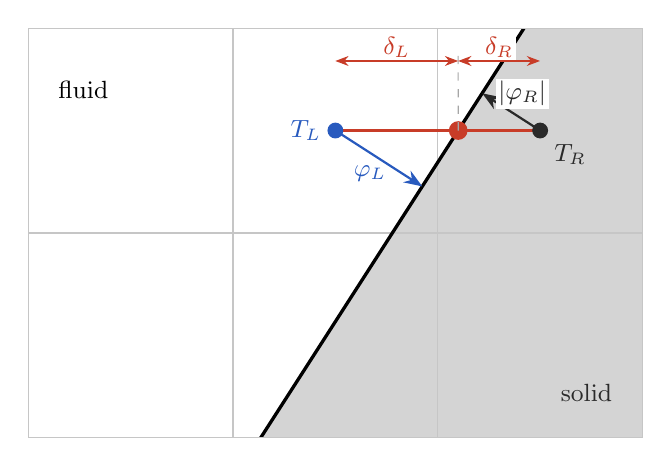
\begin{tikzpicture}[scale=2.6,>=Stealth,font=\small]
  \begin{scope}
    \clip (0,0) rectangle (3,2);
    % solid = right of the interface line through P=(2.1,1.5)
    \fill[solidcol,opacity=0.5]
       (0.943,-0.3) -- (2.743,2.5) -- (3.5,2.5) -- (3.5,-0.3) -- cycle;
    \draw[gray!45] (0,0) grid[step=1] (3,2);
    \draw[very thick] (0.943,-0.3) -- (2.743,2.5);
  \end{scope}
  \draw[gray!45] (0,0) rectangle (3,2);
  \coordinate (L)  at (1.5,1.5);
  \coordinate (R)  at (2.5,1.5);
  \coordinate (P)  at (2.1,1.5);
  \coordinate (FL) at (1.9245,1.2271);   % foot of the perpendicular from L
  \coordinate (FR) at (2.2170,1.6819);   % foot of the perpendicular from R
  % the arm and its cut point
  \draw[very thick,hot] (L) -- (R);
  \fill[hot] (P) circle (1.3pt);
  % perpendicular distances -- exactly what dwall stores
  \draw[->,thick,cold] (L) -- (FL);
  \draw[->,thick,solidcol!25!black] (R) -- (FR);
  \fill[cold] (L) circle (1.1pt);
  \fill[solidcol!25!black] (R) circle (1.1pt);
  \node[cold,anchor=east,inner sep=2pt] at (1.46,1.50) {$T_L$};
  \node[solidcol!25!black,anchor=north west,inner sep=2pt] at (2.54,1.46) {$T_R$};
  \node[cold,anchor=north east,inner sep=0pt] at (1.75,1.33) {$\varphi_L$};
  \node[solidcol!25!black,anchor=west,fill=white,inner sep=1pt]
      at (2.28,1.68) {$|\varphi_R|$};
  % the arm fractions
  \draw[dashed,gray!70] (P) -- (2.1,1.90);
  \draw[<->,hot] (1.5,1.84)
      -- node[above,fill=white,inner sep=1pt]{$\delta_L$} (2.1,1.84);
  \draw[<->,hot] (2.1,1.84)
      -- node[above,fill=white,inner sep=1pt]{$\delta_R$} (2.5,1.84);
  \node[anchor=west] at (0.10,1.70) {fluid};
  \node[solidcol!25!black,anchor=east] at (2.90,0.22) {solid};
\end{tikzpicture}
\caption{The obliquity lemma. The stored quantities $\varphi_L$, $\varphi_R$ are
perpendicular distances to the interface (blue/grey arrows) --- \emph{not}
distances along the arm. Both are shortened by the same factor
$a=\nn\cdot\ed$ relative to $\delta_L,\delta_R$, so the factor cancels in their
ratio: the level-set fraction $w$ of the arm (red) is exactly $\delta_L/h_d$ at
any interface orientation. No normal, no cut record, no per-arm geometry is
needed to evaluate the series resistance.}
\label{fig:levelset}
\end{figure}

\subsection{The scheme}

Everything the interface contributes is then one face coefficient:
\begin{equation}
  \boxed{\;
  \begin{aligned}
    &\text{if } \varphi_L\varphi_R<0:
      &&w=\frac{\varphi_L}{\varphi_L-\varphi_R},
      \qquad
      k_{\text{face}}=\left(\frac{w}{k_L}+\frac{1-w}{k_R}\right)^{-1} \\[1mm]
    &\text{else:} &&k_{\text{face}}=k_L\;(=k_R) \\[1mm]
    &\text{in both cases:} &&F=k_{\text{face}}\,\frac{T_R-T_L}{h_d}
  \end{aligned}
  \;}
  \label{eq:baseline}
\end{equation}
One sign test, one weight, one reciprocal --- inside the flux line the kernel
already has. What \eqref{eq:baseline} inherits from Sec.~\ref{sec:derivation}
comes for free:
\begin{itemize}
\item \textbf{Exact in one dimension}: it is the series resistance, so it is
      exact for a grid-aligned interface at \emph{any} cut position, and exact
      at any orientation whenever the local gradient is purely wall-normal.
\item \textbf{Conservative}: it is a face flux; $\sum C\,T\,\Delta V$ is
      conserved to round-off.
\item \textbf{Correct in both limits} (Table~\ref{tab:limits}):
      $k_R\to\infty$ is Luchini's $\lambda$, $k_R\to0$ is zero flux.
\item \textbf{Bit-exact when disabled}: an uncut face takes the else-branch,
      which is today's arithmetic unchanged.
\end{itemize}

\subsection{What it costs}
\label{sec:cost}

The dropped term is $s_t\,(k_{\text{loc}}-h_d/\Rser)$ in the face flux. The
physically meaningful error is the one in the \emph{interface-normal} flux
$q_n$, and \eqref{eq:master} gives it in closed form: the baseline solves
$a\,q_n^{\text{num}}\Rser=T_R-T_L$ instead of
$a\,q_n\Rser=T_R-T_L-h_d s_t$, so
\begin{equation}
  \boxed{\;
  \frac{q_n^{\text{num}}-q_n}{q_n}
   \;=\; \frac{h_d\,s_t}{T_R-T_L-h_d\,s_t}
   \;\approx\; \tan\theta\;
      \frac{|\grad_tT|}{|\partial_nT|},
  \qquad \cos\theta=a .
  \;}
  \label{eq:errest}
\end{equation}
Read off its properties:
\begin{itemize}
\item It vanishes identically for a grid-aligned interface ($\theta=0$) and for
      $k_s=k_f$.
\item It is set by the \emph{flow}, not by $h$: it does not converge away under
      refinement. The baseline is second order in the bulk and for
      normal-dominated interface transport, and first order in the local flux at
      obliquely cut faces carrying a tangential gradient. This is the honest
      statement, and it is the whole content of the trade.
\item In a DNS thermal boundary layer the normal gradient acts over
      $\sim1$ wall unit while $T_\Gamma$ varies over tens of wall units along
      the surface, so $|\grad_tT|/|\partial_nT|\sim10^{-2}$ and the local error
      is a few percent at strongly oblique faces.
\item $\oint_\Gamma\grad_tT\,\dd S=0$ on a closed body or a periodic wall, so
      \textbf{the surface-mean heat flux --- the Nusselt number --- is
      unaffected at leading order}. The error lives in the local, instantaneous
      distribution.
\end{itemize}

\paragraph{An a-posteriori indicator, not an assumption.}
The middle expression in \eqref{eq:errest} is composed entirely of quantities a
running simulation can form: $h_d s_t$ and $T_R-T_L$. Evaluating
\begin{equation}
  e_{\text{face}} = \frac{h_d\,s_t}{T_R-T_L}
  \qquad\text{at cut faces only}
  \label{eq:indicator}
\end{equation}
and reporting $\max|e_{\text{face}}|$ and its rms turns the premise of
Sec.~\ref{sec:baseline} into a \emph{measured} quantity. And since evaluating
\eqref{eq:indicator} requires exactly the $s_t$ that the correction needs,
switching the correction on is free once the indicator is implemented ---
Sec.~\ref{sec:escalation}.

\subsection{Everything from one stored field}
\label{sec:onefield}

The signed distance is $\varphi=\pm\,\code{dwall}$, the sign taken from the
existing solid marker. \code{dwall} is already computed at \emph{every cell
centre including ghosts}, at the \code{VAR\_P} position where the scalar lives,
for the analytic path (\code{fill\_body\_distance\_analytic}) and for the file
path (\code{dwall\_blocks}, written by default by \code{moby\_prepare} and read
by \code{read\_dwall\_blocks}). Table~\ref{tab:needs} is the consequence.

\begin{table}[htbp]
\centering
\caption{What each variant needs. The baseline adds \emph{no} stored data to a
case file that already carries \code{dwall\_blocks}; the escalation adds
arithmetic, not data.}
\label{tab:needs}
\small
\begin{tabular}{@{}lll@{}}
\toprule
quantity & baseline \eqref{eq:baseline} & escalation \eqref{eq:main} \\
\midrule
cut fraction $w$ & $\varphi_L/(\varphi_L-\varphi_R)$ & same \\
direction cosine $a$ & not used & $(\varphi_L-\varphi_R)/h_d$, Eq.~\eqref{eq:afree} \\
normal $\nn$ & not used & $\grad\varphi$ (unit; central differences) \\
$\partial_nT$ & not used & $\grad\varphi\cdot\grad T$, ordinary differences \\
$s_t$ & not used & $\ed\cdot\grad T-a\,(\grad\varphi\cdot\grad T)$ \\
volume fraction $\phi$ & transients only & $\mathrm{clip}(\tfrac12+\varphi_c/h)$ \\
\midrule
\textbf{new case-file datasets} & \textbf{none} & \textbf{none} \\
\bottomrule
\end{tabular}
\end{table}

The line that matters is the last one. Because $\varphi$ is a true distance
function, $|\grad\varphi|=1$ and $\grad\varphi$ \emph{is} the unit normal --- the
same identity the RANS wall functions already exploit for \code{sst\%wnorm}. So
the normal, the obliquity and the normal derivative are all obtainable from
central differences of $\varphi$ and $T$: \textbf{the entire method, baseline
and escalation, requires exactly one extra stored field, and that field already
exists.} No \code{cut\_arms\_blocks} dataset, no per-arm bisection records, no
precomputed least-squares weights, no volume-fraction tiles.

\subsection{Curvature, grazing arms, and when to distrust \texorpdfstring{$w$}{w}}
\label{sec:wcaveats}

Equation~\eqref{eq:w} is exact for a plane. For a curved interface $\varphi_L$
and $\varphi_R$ are distances to \emph{different} nearest points, and the zero
of the linear interpolant is displaced by $O(\kappa h^2/a)$, i.e.\ $w$ carries a
relative error $O(\kappa h/a)$ with $\kappa$ the local curvature. At DNS
resolution with \code{refine\_body} clustering cells on the surface,
$\kappa h\ll1$ by construction --- but note the $1/a$: the estimate degrades for
\emph{grazing} arms, those nearly tangent to the surface. Such arms carry little
of the interface flux, and the practical guard is to fall back to the plain
harmonic mean when $a$ falls below a threshold. If exactness in $w$ is ever
required, the per-arm bisection of \code{add\_neighbor\_coeff} supplies it
directly --- at the price of the per-arm dataset the baseline exists to avoid.

\subsection{The escalation path}
\label{sec:escalation}

If \eqref{eq:indicator} says the local flux error matters, the route back to the
formally second-order scheme is a single additional term at the \emph{same}
face,
\begin{equation}
  F = k_{\text{face}}\frac{T_R-T_L}{h_d}
      + s_t\left(k_{\text{loc}}-k_{\text{face}}\right),
\end{equation}
with $s_t$ from Table~\ref{tab:needs} --- the correction is already computed if
the indicator is running. Nothing about the data layout, the face loop, the
conservation argument or the limits changes. This is why the baseline is a
\emph{starting point} rather than a different method: it is \eqref{eq:main} with
one term switched off, and the switch is a runtime decision informed by a
measurement.

%======================================================================
\section{The discrete scheme}
%======================================================================

\subsection{Face loop}

The existing kernel already computes six face fluxes per cell. The scheme is a
\emph{branch on the face type}:

\begin{center}
\begin{tabular}{@{}ll@{}}
\toprule
face type & flux \\
\midrule
uncut, both cells fluid & unchanged: $D_{\text{face}}(T_R-T_L)/\Delta$,
                          $D=\tfrac{1}{\mathrm{Re}\,\mathrm{Pr}}+\tfrac{\nu_t}{\mathrm{Pr}_t}$\\
uncut, both cells solid & $\kappa_s\,(T_R-T_L)/(\mathrm{Re}\,\mathrm{Pr}\,\Delta)$, no eddy part\\
cut ($\varphi_L\varphi_R<0$) & Eq.~\eqref{eq:baseline}: $w$ from the two signed
                          distances, then $k_{\text{face}}$ \\
\code{FACE\_CLOSED}     & masked, as today\\
\bottomrule
\end{tabular}
\end{center}

Fluid--fluid faces are byte-identical to the current arithmetic, so the feature
is bit-exact when disabled \emph{and} away from the body when enabled. The cell
update divides the flux divergence by the local capacity $C$
(Eq.~\eqref{eq:onefield}).

\subsection{Convection}

The convective flux must be \emph{hard-masked} on every face whose staggered
velocity node is solid and on every cut face. Physically $\boldsymbol{u}\cdot\nn=0$
on $\Gamma$, so masking is consistent to second order. Relying on the penalised
velocity being ``small'' is not acceptable here: unlike a passive scalar in a
Dirichlet body, the solid now carries a genuine temperature field that must not
be advected. Note also that near the interface the diffusive term dominates the
convective one (the argument of \cite{luchini2025}, \S3.1, transfers verbatim
from momentum to temperature), which is what licenses correcting the diffusive
operator alone.

\subsection{The tangential gradient $s_t$ (escalation only)}

The baseline never forms $s_t$; this subsection applies to the indicator
\eqref{eq:indicator} and to the escalation \eqref{eq:main}.

Two constructions are available, in increasing cost:
\begin{enumerate}
\item \textbf{From $\varphi$ and ordinary differences} (Table~\ref{tab:needs}):
      $\nn=\grad\varphi$, $a$ from \eqref{eq:afree}, and
      $s_t=\ed\!\cdot\!\grad T-a\,(\grad\varphi\!\cdot\!\grad T)$ with both
      gradients from the central differences the kernel already forms. No new
      data, no new stencil. This is the recommended construction.
\item \textbf{Same-side least squares} over the $3^3$ neighbourhood
      (Fig.~\ref{fig:stencil}), if the ordinary differences prove too
      contaminated by the interface --- they straddle it, and $\grad T$ is
      discontinuous there. The $3^3$ neighbourhood, and no more, is exactly what
      the 26-neighbour halo exchange provides; the weights are geometry-only and
      can be precomputed.
\end{enumerate}
Because the required quantity is the \emph{continuous} tangential component,
construction 1 is forgiving in a way a normal-derivative estimate would not be.
If two estimates are available, prefer the side with the \emph{larger}
conductivity: the low-conductivity side carries the steeper, noisier gradient.
(This is the freedom noted in \cite{ejiim2000}, footnote~1: the jump relations
can be written in terms of either one-sided limit, and the formulations are not
equally well conditioned.)

\begin{figure}[htbp]
\centering
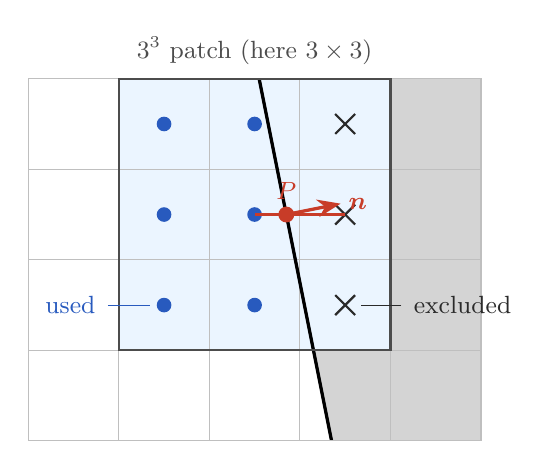
\begin{tikzpicture}[scale=1.15,>=Stealth,font=\small]
  \begin{scope}
    \clip (0,0) rectangle (5,4);
    \fill[solidcol,opacity=0.5] (3.35,0) -- (5,0) -- (5,4) -- (2.55,4) -- cycle;
    % the 3x3 patch around the cut cell (centre at (2.5,2.5))
    \foreach \x in {1,2,3} \foreach \y in {1,2,3}
       \fill[fluidcol] (\x,\y) rectangle ++(1,1);
    \draw[gray!50] (0,0) grid[step=1] (5,4);
    \draw[very thick] (3.35,0) -- (2.55,4);
  \end{scope}
  \draw[gray!50] (0,0) rectangle (5,4);
  \draw[thick,black!70] (1,1) rectangle (4,4);
  % same-side (fluid) centres of the patch
  \foreach \p in {(1.5,1.5),(2.5,1.5),(1.5,2.5),(2.5,2.5),(1.5,3.5),(2.5,3.5)}
      \fill[cold] \p circle (2.3pt);
  % opposite-side centres, excluded
  \foreach \p in {(3.5,1.5),(3.5,2.5),(3.5,3.5)}
      {\draw[solidcol!25!black,thick] \p ++(-0.11,-0.11) -- ++(0.22,0.22);
       \draw[solidcol!25!black,thick] \p ++(-0.11,0.11) -- ++(0.22,-0.22);}
  % the cut arm of interest and the interface point
  \draw[thick,hot] (2.5,2.5) -- (3.5,2.5);
  \fill[hot] (2.85,2.5) circle (2.5pt);
  \node[hot,above=2pt] at (2.85,2.5) {$P$};
  \draw[->,very thick,hot] (2.85,2.5) -- ++(0.60,0.12) node[right=-1pt]{$\nn$};
  \node[cold,anchor=east] at (0.85,1.5) {used};
  \draw[cold,thin] (0.88,1.5) -- (1.35,1.5);
  \node[solidcol!25!black,anchor=west] at (4.15,1.5) {excluded};
  \draw[solidcol!25!black,thin] (4.12,1.5) -- (3.68,1.5);
  \node[black!70,anchor=south] at (2.5,4.05) {$3^3$ patch (here $3\times3$)};
\end{tikzpicture}
\caption{Same-side stencil for the tangential gradient at the interface point
$P$ of one cut arm (red). $\grad T^{-}|_P$ is obtained by weighted least
squares over the same-side cells of the $3^3$ patch around the cut cell; the
weights depend on geometry only and are precomputed in \code{moby\_prepare}.
Only the $3^3$ neighbourhood is used, which is exactly what the existing
26-neighbour halo exchange delivers --- EJIIM's wider one-sided operators are
deliberately not adopted. Since $\grad_tT$ is continuous, a modest estimate
suffices.}
\label{fig:stencil}
\end{figure}

\subsection{Capacity at cut cells}

A cut cell contains both materials, so its volumetric capacity is
\begin{equation}
  C_{\text{cell}} = \phi + (1-\phi)\,C_s,
  \qquad
  \phi = \frac{|\text{cell}\cap\Omega_f|}{|\text{cell}|},
\end{equation}
with $\phi$ computed once at preprocessing (Fig.~\ref{fig:capacity}). This is
irrelevant for steady problems and required for second-order \emph{transients};
it also makes the global capacity $\sum C_{\text{cell}}\Delta V$ exact.

\begin{figure}[htbp]
\centering
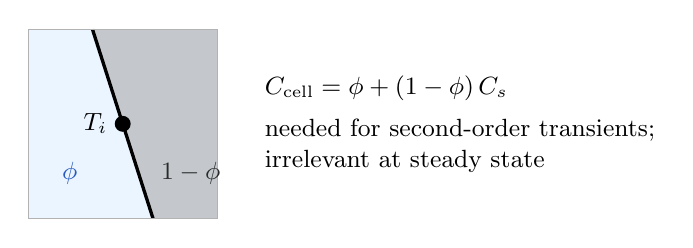
\begin{tikzpicture}[scale=2.4,>=Stealth,font=\small]
  \fill[fluidcol] (0,0) rectangle (1,1);
  \fill[solidcol,opacity=0.6] (0.66,0) -- (1,0) -- (1,1) -- (0.34,1) -- cycle;
  \draw[very thick] (0.66,0) -- (0.34,1);
  \draw[gray!60] (0,0) rectangle (1,1);
  \fill[black] (0.5,0.5) circle (1.2pt);
  \node[anchor=east] at (0.47,0.5) {$T_i$};
  \node[cold] at (0.22,0.24) {$\phi$};
  \node[solidcol!25!black] at (0.86,0.24) {$1-\phi$};
  \node[right,align=left] at (1.20,0.5)
    {$C_{\text{cell}}=\phi+(1-\phi)\,C_s$\\[1.5mm]
     needed for second-order transients;\\ irrelevant at steady state};
\end{tikzpicture}
\caption{Fluid volume fraction of a cut cell.}
\label{fig:capacity}
\end{figure}

%======================================================================
\section{Stability and time integration}
\label{sec:stability}
%======================================================================

\subsection{The conjugate interface is not stiff}

This is a genuinely useful structural result. Since
$\delta_L+\delta_R=h_d$,
\begin{equation}
  \Rser=\frac{\delta_L}{k_L}+\frac{\delta_R}{k_R}
       \;\ge\; \frac{h_d}{\max(k_L,k_R)} \;>\;0
  \qquad\text{for \emph{every} cut position.}
\end{equation}
The $\delta\to0$ singularity that forces the implicit treatment
\eqref{eq:luchini-B} in the Dirichlet case simply \emph{does not exist} in the
conjugate case: as the interface approaches one cell centre, the resistance of
that sub-segment vanishes but the other one takes over. Combined with the fact
that cells retain their full volume (this is an embedded-boundary, not a
cut-cell, method), there is no small-cell problem and no exponential integrator
is needed at the interface. Figure~\ref{fig:stiffness} contrasts the two cases.

\begin{figure}[htbp]
\centering
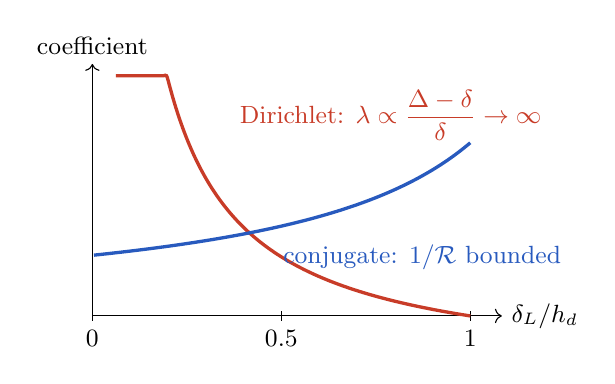
\begin{tikzpicture}[scale=1.0]
  \draw[->] (0,0) -- (5.2,0) node[right,font=\small] {$\delta_L/h_d$};
  \draw[->] (0,0) -- (0,3.2) node[above,font=\small] {coefficient};
  \foreach \x/\l in {0/0,2.4/0.5,4.8/1} \draw (\x,0.06)--(\x,-0.06) node[below,font=\small]{\l};
  % Luchini lambda ~ (1-d)/d  -> diverges as d->0
  \draw[very thick,hot,domain=0.30:4.8,samples=120,smooth]
     plot (\x,{min(3.05, 0.75*(4.8-\x)/(\x))});
  \node[hot,font=\small,anchor=west] at (1.75,2.55)
     {Dirichlet: $\lambda\propto\dfrac{\Delta-\delta}{\delta}\to\infty$};
  % conjugate 1/R : bounded
  \draw[very thick,cold,domain=0.02:4.8,samples=120,smooth]
     plot (\x,{2.2/((\x/4.8)+(1-\x/4.8)/0.35)*1.0});
  \node[cold,font=\small,right] at (2.3,0.75) {conjugate: $1/\Rser$ bounded};
\end{tikzpicture}
\caption{Coefficient magnitude versus cut position. The Dirichlet
immersed-boundary coefficient $\lambda$ diverges as the wall approaches a node
(hence Eq.~\eqref{eq:luchini-B}); the conjugate face conductance $1/\Rser$ stays
bounded by $\max(k_L,k_R)/h_d$ for every cut position.}
\label{fig:stiffness}
\end{figure}

\subsection{What does constrain the time step}

The solid diffusivity. The explicit diffusive limit becomes
\begin{equation}
  \Delta t \;\le\; \frac{h^{2}}{2\,n_{\text{dim}}\,\max(\alpha_f,\alpha_s)},
  \qquad \frac{\alpha_s}{\alpha_f}=\frac{\kappa_s}{C_s},
\end{equation}
and $\alpha_s/\alpha_f\sim10^{2}$ (a metal against water) is entirely ordinary.
Three escalation levels, in order:
\begin{enumerate}
\item extend the existing P\'eclet limiter
      (\code{precompute\_peclet\_rate}) to take the maximum over materials, and
      accept the cost;
\item point-implicit the solid diagonal using \emph{Luchini's} factor
      $B(\lambda\Delta t)$ of Eq.~\eqref{eq:luchini-B} verbatim --- the same
      formula, reused for the solid interior rather than for the wall;
\item implicit solid diffusion on the damped-Jacobi / Chebyshev machinery that
      \code{pressure\_solver.f90} already owns.
\end{enumerate}
Start at (1); escalate only on measured evidence.

\subsection{Explicit stability of the tangential term}

The correction $s_t\,(k_{\text{loc}}-h_d/\Rser)$ is an explicit spatial operator
evaluated on the current field --- it is not a lag. Its magnitude relative to the
principal diffusive term grows with the conductivity contrast, so it may cost
some time step at extreme contrast. This is a quantity to \emph{measure}
(gate~2 below at $\kappa_s=10^{3}$), with under-relaxation or clipping of the
correction as the fallback.

%======================================================================
\section{Geometric data and where it is produced}
%======================================================================

Table~\ref{tab:needs} already gave the answer: \textbf{nothing new is produced},
because \code{dwall} is produced today. What remains is to state precisely what
that field is and what must be arranged around it.

\paragraph{What \code{dwall} is.}
An \emph{unsigned} Euclidean distance to the immersed surface, evaluated at
every cell centre \emph{including ghost cells} at the \code{VAR\_P} position ---
the scalar's own location --- for both geometry paths:
\begin{center}
\begin{tabular}{@{}ll@{}}
\toprule
analytic geometry & \code{fill\_body\_distance\_analytic} (rans.f90), from the
                    \code{isInBody} indicator alone \\
file geometry     & \code{dwall\_blocks}, written by default by
                    \code{moby\_prepare}, read by \code{read\_dwall\_blocks} \\
\bottomrule
\end{tabular}
\end{center}
It is per leaf, at that leaf's own level, and it is exact to
\code{[rans] dwall\_tol}. The sign is supplied by the existing solid marker
(the cell-centred IBM coefficient above its solid threshold, equivalently
\code{wallcell}); $\varphi=\pm\,\code{dwall}$.

\paragraph{Two arrangements are required, neither of them new data.}
\begin{enumerate}
\item \textbf{Availability without RANS.} Today the distance state is built only
      when a \code{[rans]} section is present (the T1 hook). A conjugate run is
      typically a DNS with no turbulence model, so the build must also be
      triggered by \code{ibm\_wall = conjugate}. For file geometry this is a
      read of a dataset that is already in the case file; for analytic geometry
      it is a call to a routine that already exists.
\item \textbf{A ghost-inclusive sign.} $\varphi$ is needed on the halo layer so
      that cut faces on a block boundary see both signs. \code{dwall} is already
      ghost-inclusive; the solid marker must be too.
\end{enumerate}

\paragraph{What is NOT needed, and why that matters.}
\code{add\_neighbor\_coeff} bisects to the cut point and then \emph{sums the six
arms away} into one scalar $\lambda$ --- exactly right for Dirichlet
penalisation, and useless for CHT. An earlier draft of this note therefore
proposed a new per-leaf \code{cut\_arms\_blocks} dataset carrying per-arm cut
distances, normals, volume fractions and least-squares weights. The obliquity
lemma \eqref{eq:w} removes the need for all of it: the cut fraction, the
direction cosine and the normal all follow from a field that is already written,
already read, and already validated (the T1 gates measured it against closed-form
references to $10^{-11}$). \textbf{No new dataset, no new preprocessing stage, no
case-file format change, and no ``re-run \code{moby\_prepare}'' error path.}

%======================================================================
\section{Two cheaper routes to check first}
\label{sec:cheaper}
%======================================================================

Before implementing anything above, two questions can remove the problem
entirely. Both are worth asking of every target case.

\paragraph{1. Can the interface be made grid-aligned?}
If the conducting wall is a plane --- a channel with conducting slabs, the
existing \code{les\_ibm} geometry with its wall moved onto a cell face --- then
put the interface \emph{on} a face. Then $w=\tfrac12$, $k_{\text{face}}$ is the
plain harmonic mean, and \eqref{eq:baseline} is the textbook variable-coefficient
finite-volume scheme with \textbf{no immersed-boundary involvement and no
approximation of any kind}: second order, exactly conservative, exact interface
condition. This is how the canonical conjugate-DNS channel studies are set up,
and it costs nothing but a grid choice. Only genuinely non-grid-aligned geometry
needs the machinery of Sec.~\ref{sec:baseline}, and even that machinery is one
face coefficient.

\paragraph{2. Does the solid need to be solved at all?}
If the solid is thin compared with the thermal penetration depth, or so
conductive that it is effectively isothermal, or so slow that it is quasi-steady
on the fluid time scale, then replace it by a Robin condition
\begin{equation}
  k_f\,\partial_nT = h_{\text{eff}}\,(T_\Gamma-T_{\text{ref}})
\end{equation}
with $h_{\text{eff}}$ from a one-dimensional solid model. No solid field, no
buried-block constraint, no solid time-step limit
(Sec.~\ref{sec:stability}), no capacity fraction --- and for many conjugate
questions (how finite wall conductance changes the near-wall temperature
statistics) the physics enters through the same two dimensionless groups as the
full problem. This is a modelling decision, not a numerical one, and it should
be made deliberately rather than by default.

%======================================================================
\section{Alternatives considered and rejected}
%======================================================================

\begin{description}
\item[Full EJIIM augmented system with Schur complement and GMRES
      (\cite{ejiim2000} \S6.3).] The faithful route, and unnecessary here: an
      explicit march makes every jump computable (Sec.~3). It is also
      incompatible with block decomposition, $2\!:\!1$ refinement and GPU
      offload. It \emph{is} worth building as a standalone two-dimensional
      reference implementation for the manufactured-solution gates --- the same
      role \code{mobygeom} plays as a cross-implementation reference.
\item[Liouville transformation (\cite{ejiim2000} \S4.4).] Solving for
      $\tilde u=\sqrt{\beta}\,u$ makes the \emph{primary variable}
      discontinuous, $\jump{\tilde u}=(\rho^{-1/2}-1)\tilde u^-$. Wrong trade for
      a variable that is transported, written to snapshots and restarted.
\item[Normal-probe ghost-cell conjugate IBM.] Requires the same same-side
      interpolation but \emph{replaces} the stencil rather than correcting it,
      losing conservation-by-telescoping and the bit-exact-when-disabled
      property.
\item[A precomputed per-arm cut dataset.] Superseded by the obliquity lemma
      \eqref{eq:w}: everything it would carry follows from \code{dwall}, which
      is written and read today. Retained only as the fallback if the
      $O(\kappa h/a)$ curvature error in $w$ (Sec.~\ref{sec:wcaveats}) is ever
      shown to bind.
\end{description}

\noindent
Note what is \emph{not} on this list: distance-weighted harmonic averaging
alone. That is Eq.~\eqref{eq:main} with $s_t$ dropped, and it is now the
recommended baseline (Sec.~\ref{sec:baseline}) --- not because it is formally
second order at oblique faces (Sec.~\ref{sec:counting} proves it cannot be) but
because at DNS resolution its error is quantified by \eqref{eq:errest},
measurable by \eqref{eq:indicator}, mean-cancelling over a closed surface, and
removable by one extra term if a measurement demands it.

%======================================================================
\section{Validation ladder}
%======================================================================

The gates are stated in full, with expected outcomes, in
\code{docs/next\_session\_conjugate.md}, \S10. In brief:
\begin{enumerate}
\item \textbf{Disabled} $\Rightarrow$ bit-exact (\code{-Mnofma},
      \code{max\_abs 0}) on the standard seven-case suite, CPU and GPU.
\item \textbf{One-dimensional two-material slab}, cut position swept through a
      full cell, $\kappa_s\in\{10^{-2},1,10,10^{3}\}$: the baseline
      \eqref{eq:baseline} must be \emph{exact} (the steady solution is piecewise
      linear and the series resistance is then exact). This gate also validates
      $w$ from the signed distances against the analytic cut position.
\item \textbf{Limits}: $\kappa_s\to\infty$ reproduces the Dirichlet mode,
      $\kappa_s\to0$ the adiabatic mode.
\item \textbf{Conservation}: $\sum C\,T\,\Delta V$ drift at round-off in an
      insulated composite box.
\item \textbf{Oblique plane interface}, manufactured solution at
      $30^\circ$/$45^\circ$ with a \emph{controlled} ratio
      $|\grad_tT|/|\partial_nT|$, $\kappa_s\in\{10,10^{3}\}$: \emph{the gate that
      decides how far to go}. Measure the interface-flux error against that
      ratio and against $h$, and check it against the prediction
      \eqref{eq:errest} and the indicator \eqref{eq:indicator}. At DNS-like
      ratios ($\sim10^{-2}$) the baseline is expected to be adequate and the
      escalation unnecessary; at $O(1)$ ratios the baseline should stall near
      first order and the escalation recover second.
\item \textbf{Cylindrical shell}, exact logarithmic solution: curved interface;
      isolates the $O(\kappa h/a)$ error of Sec.~\ref{sec:wcaveats} in the
      interface flux (Nusselt).
\item \textbf{Transient} two-material slab with a capacity jump, against the
      analytic solution.
\item \textbf{Production}: the existing off-grid plane-wall case
      \code{validation/channel\_interface/les\_ibm/} made conducting --- its
      walls sit mid-cell, so the cut fractions are non-trivial while the
      interface stays grid-aligned, making it a clean regression \emph{and} a
      case in which the baseline is exact.
\end{enumerate}

%======================================================================
\begin{thebibliography}{9}
\bibitem{luchini2025}
P.~Luchini, D.~Gatti, A.~Chiarini, F.~Gattere, M.~Atzori, M.~Quadrio,
\emph{A simple and efficient second-order immersed-boundary method for the
incompressible Navier--Stokes equations},
J.~Comput.\ Phys.\ \textbf{539} (2025) 114245.
\bibitem{ejiim2000}
A.~Wiegmann, K.~P.~Bube,
\emph{The explicit-jump immersed interface method: finite difference methods for
PDEs with piecewise smooth solutions},
SIAM J.~Numer.\ Anal.\ \textbf{37}(3) (2000) 827--862.
\bibitem{cipelli2025}
S.~Cipelli, A.~Chiarini, M.~Quadrio, D.~Gatti, P.~Luchini,
\emph{Handling geometric singularities efficiently with the immersed-boundary
method: application to riblets}, preprint (2025)
(\code{literature/cipelli-2025.pdf}).
\end{thebibliography}

\end{document}
